%===============================================================================
% Brno University of Technology
% Faculty of Information Technology
% Academic year: 2018/2019
% Bachelor thesis: Monitoring Pedestrian by Drone
% Author: Vladimir Dusek
%===============================================================================

\chapter{Detekce objektů v~obraze}
\label{chap_2}

Detekce objektů je počítáčová technologie z~oblasti počítačového vidění (\textit{computer vision}) a zpracování obrazu (\textit{image processing}). Zabývá se rozpoznáním objektů v~digitálních obrázcích či videích a jejich následným zařazením (klasifikací) do předem definovaných kategorií (tříd). Může se jednat například o~detekci lidí, automobilů, zvířat či v~podstatě čehokoliv jiného, záleží pouze na množině trénovacích dat. O~trénování více v~sekci~\ref{sec_training_neural_network}.

V~poslední době zažívá sféra detekce objektů v~obraze velký rozmach a vzbuzuje značný zájem v~oblasti umělé inteligence. S~rozvojem architektury konvolučních neuronových sítí, za kterými stojí velké množství trénovacích dat a pokročilé výpočetní technologie, se schopnost strojů rozpoznávat objekty ve scénách výrazně zlepšila. Počítače nyní, za určitých specifických nastavení, dokáží v~některých konkrétních úlohách dokonce překonat člověka, například v~rozpoznávání lidských tváří~\cite{paperSurpassingHuman}.

Již dnes lze najít velké množství konkrétních využití detekce objektů. Například optické rozpoznávání vytišťených či ručně psaných znaků lze využít pro automatické rozeznávání státních poznávacích značek aut na záznamech z~kamer či digitalizaci různých typů tištěných dokumentů. V~míčových sportech lze využít detekci objektů pro sledování míče. Na sociálních sítích je zase implementována detekce lidských obličejů pro rozpoznávání tváří uživatelů na fotografiích. Další příklad využití detekce objektů jsou samořídící auta. Ty jsou sice otázkou až blízké budoucnosti, je ale zřejmé, že musí umět velmi spolehlivě rozeznávat veškeré objekty kolem sebe (jiné auto, člověk, semafor, ...) a podle toho reagovat.

%===============================================================================

\section{Proces detekce objektů}
\label{sec_process_object_detection}

Kompletní proces detekce objektů je běžně rozdělen do několika fází. Za úplně první krok může být považováno pořízení vstupních digitálních obrazových dat fotoaparátem nebo videokamerou. Získaná data jsou následně předzpracována jednoduchými úpravami (\textit{preprocessing}). Například se jedná o~změnu rozlišení, zvýraznění hran objektů, úpravy jasu, kontrastu, normalizace barev apod. Druh předzpracování záleží na konkrétní metodě detekce, některé jej nevyužívají vůbec.

Dalším krokem je segmentace obrazu, kdy jsou vybrána místa, kde by se potenciálně mohl vyskytovat nějaký hledaný objekt. Nejjednodušší metody pracují s~oknem, které se s~určitým krokem posouvá po obraze a výřezy jsou předávány klasifikátoru. Pro detekci objektů s~různým poměrem stran a orientací je nutné použít okno opakovaně s~různými parametry. Problém těchto metod je velký počet výřezů, což má za následek značné výpočetní nároky. V~dnešní době valná většina detektorů funguje na základě neuronových sítí. Ty jsou schopny selektivně vybírat vhodné hraniční oblasti, a tím výrazně snížit počet výřezů.

Posledním krokem je klasifikace objektu. Z~vyříznuté oblasti je extrahován příznakový vektor, který je porovnán se vzorovými příznaky jednotlivých tříd. Příznaky slouží jako popis samostatného objektu. Mohou jimi být například barva, struktura nebo tvar. U~neuronových sítí je extrakce příznaků prováděna pomocí konvolučních vrstev. Porovnávání příznaků provádí klasifikátor, ten rozhodne, zda se jedná o~objekt z~předem známých kategorií (tříd).

\begin{figure}[H]
    \centering
    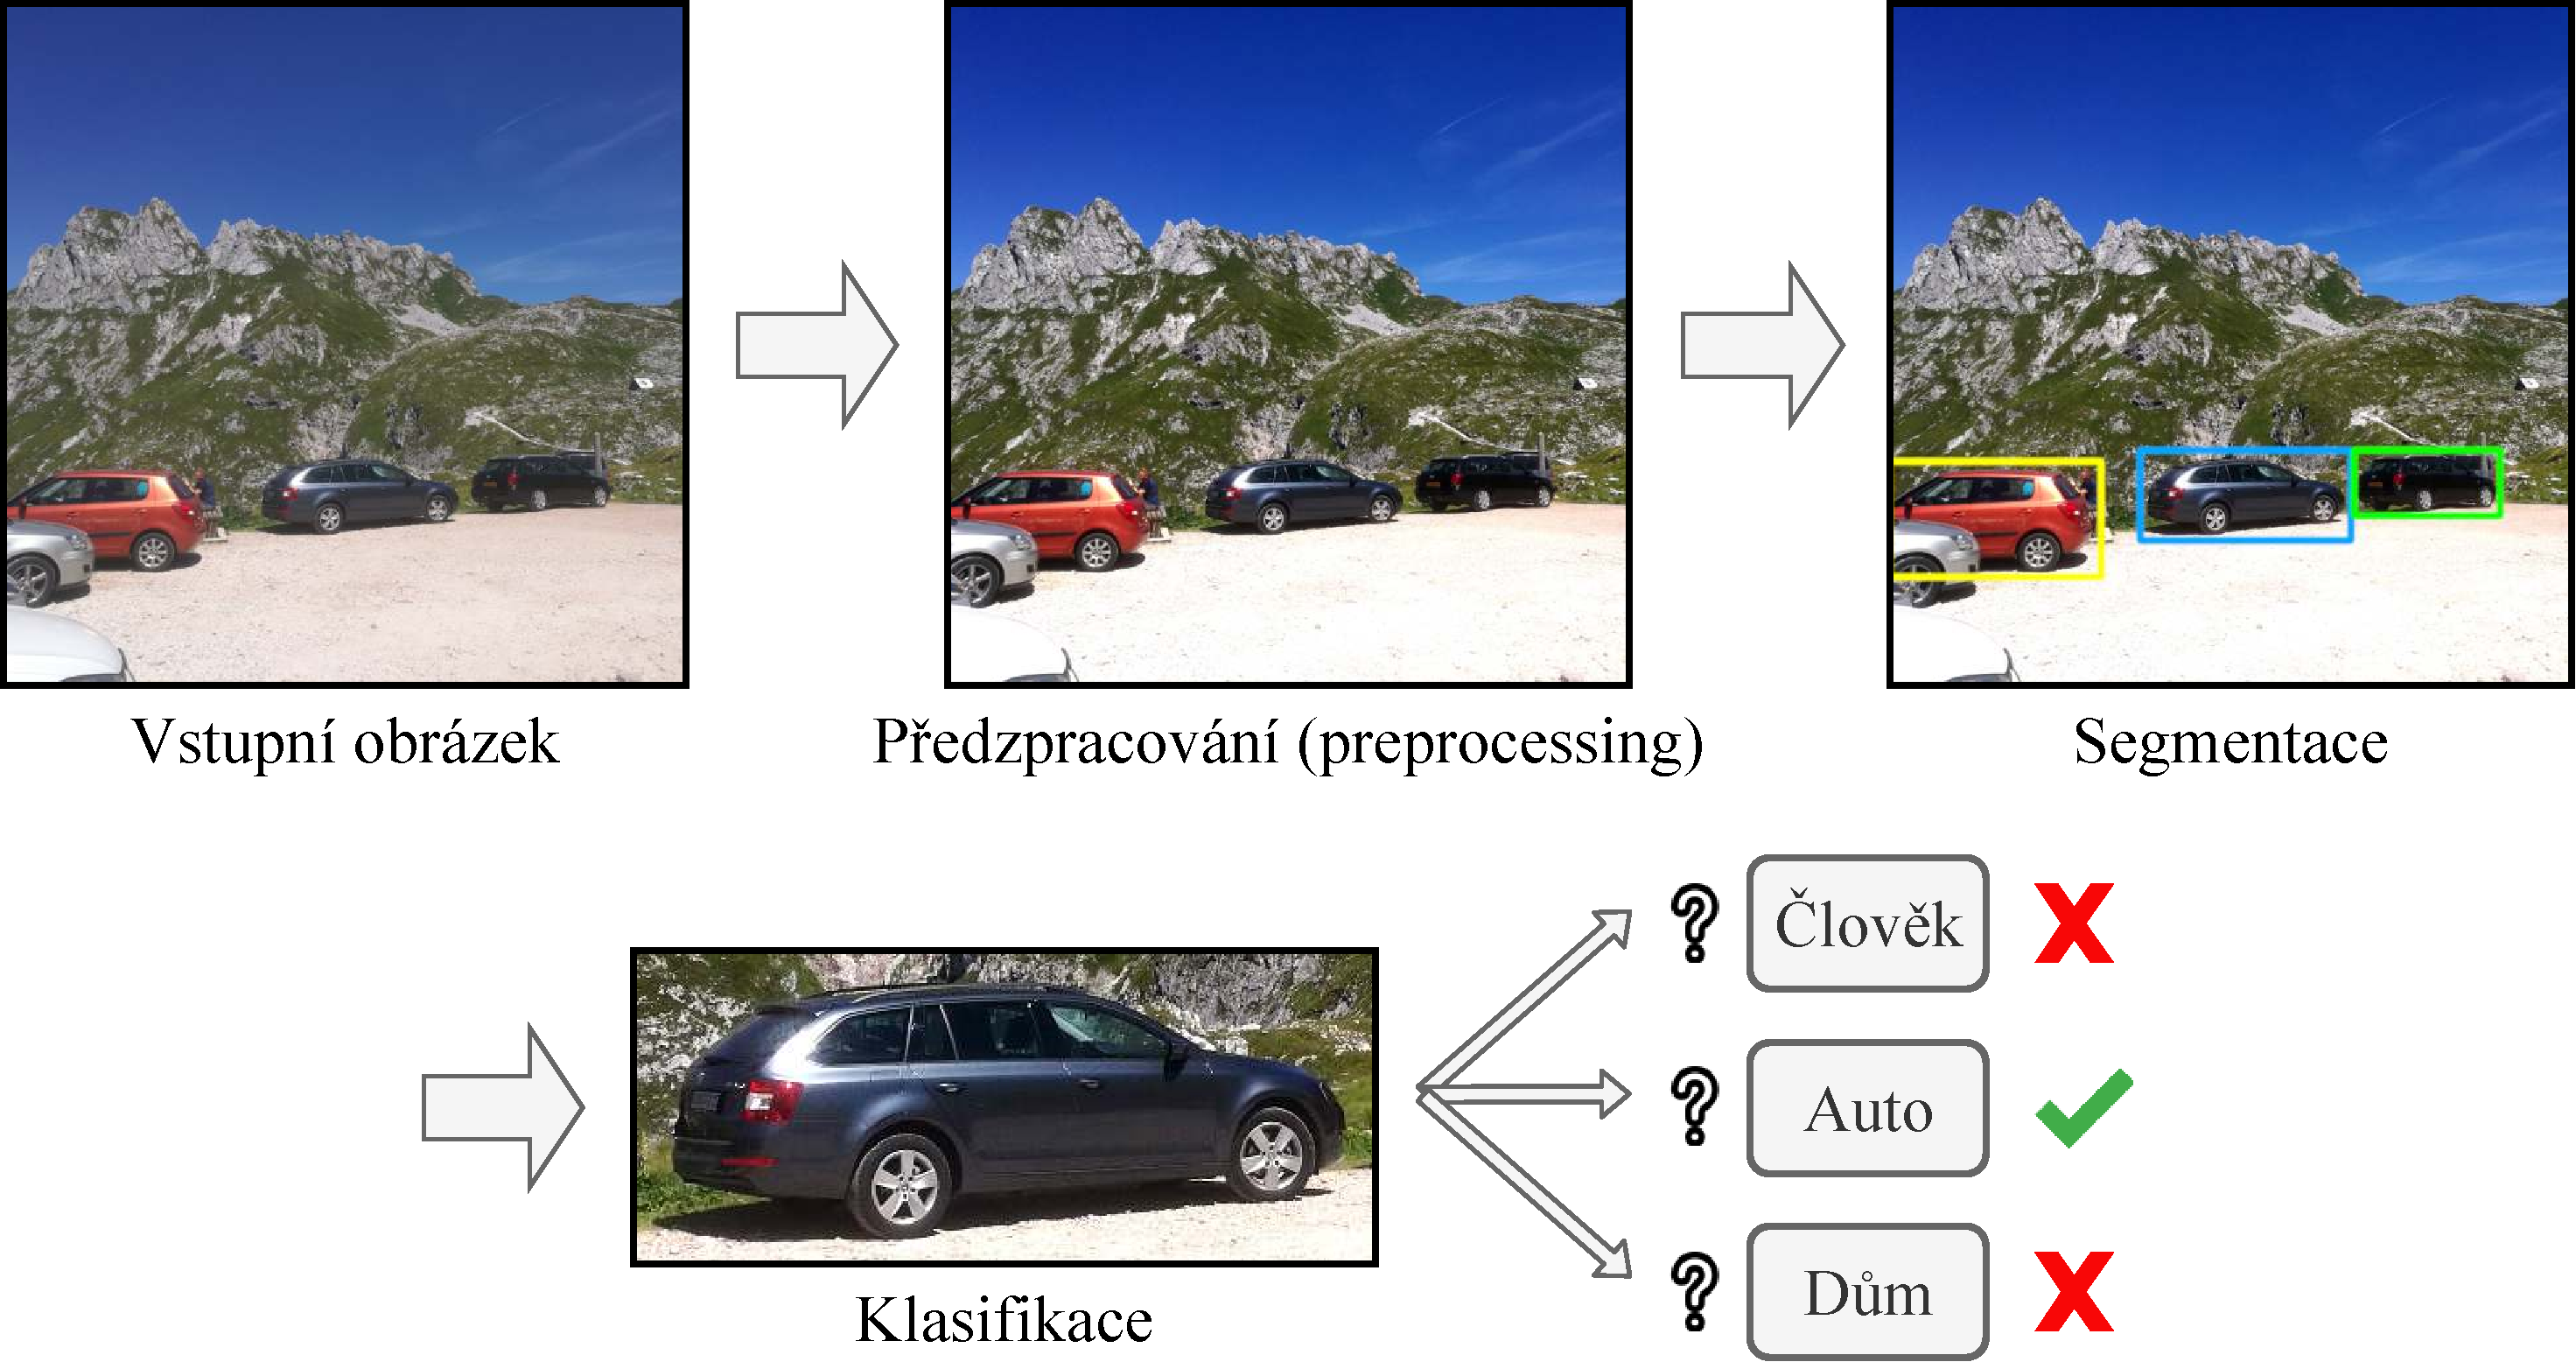
\includegraphics[width=.99\linewidth]{object_detection_schema.pdf}
    \caption[Schéma procesu detekce objektů v~obraze]{Schéma procesu detekce objektů v~obraze.}
    \label{fig_object_detection_schema}
\end{figure}

%===============================================================================

\section{Klasifikační algoritmy}
\label{sec_classification_algorithms}

Algoritmy pro detekci objektů v~obraze je možné rozdělit podle toho, jakým způsobem jsou jim nastaveny příznaky (\textit{features}). Algoritmy se snaží tyto příznaky v~datech hledat a na jejich základě provádět klasifikaci. První jsou klasifikátory, které mají příznaky předprogramované (\textit{hand coded}). Mají zaměření na konkrétní typ dat a přeučit je na jiné vyžaduje přeprogramování příznaků. Tímto typem klasifikátorů se zabývá tato sekce. Druhým typem jsou klasifikátory, jejichž příznaky jsou dynamicky upravovány trénováním. Po naprogramování nemají žádné zaměření, a ještě nejsou schopny klasifikovat žádná data. Tuto schopnost získají až po procesu natrénování na trénovacích datech. Mezi tento typ klasifikátorů patří neuronové sítě, viz sekce~\ref{sec_neural_networks}.

%-------------------------------------------------------------------------------

\subsection*{Algoritmus Viola--Jones}

Ačkoliv se lidé oblasti detekce objektů v~obraze pomocí počítačů věnují již od 60.~let 20.~století, dlouho se nedařilo přijít s~výsledky, které by bylo možné k~něčemu reálně využít. Zlom nastal až v~novém tisíciletí, kdy v~roce~2001 přišli Paul Viola a Michael Jones s~algoritmem, který pojmenovali po sobě samých~\cite{paperViolaJones}. Algoritmus byl primárně navržen pro detekci obličejů, lze jej však upravit pro detekci různých objektů s~výraznými hranami.

Demonstrační aplikace, kterou Paul Viola a Michael Jones představili, byla schopná v~reálném čase detekovat obličeje na videu z~webkamery. Byla zde jistá omezení: Celá plocha obličeje musela směřovat přesně k~fotoaparátu a obličej nesměl být nijak nakloněn. I~přesto se jednalo v~té době o~revoluční objev, který demonstroval potenciál počítačového vidění. Algoritmus byl brzy implementován do knihovny OpenCV a stal se synonymem pro detekci obličejů.

Algoritmus využívá toho, že lidské tváře sdílí podobné rysy. Například oblast očí je obvykle tmavší než líce, nosní přepážka je zase světlejší než oblast očí. Využívá také celkové kompozice obličeje, pozici a velikosti očí, pusy a nosu. Snímek je na začátku zpracování převeden do stupně šedi (\textit{greyscale}), kde tyto vlastnosti lépe vyniknou. Jejich míra shody je poté zjišťována pomocí Haarových příznaků.

\begin{figure}[H]
    \centering
    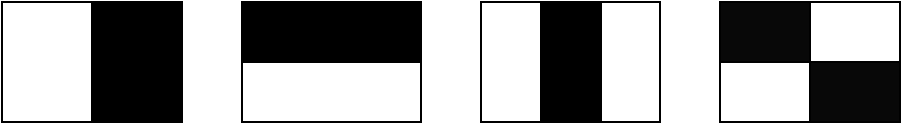
\includegraphics[width=.95\linewidth]{haar_features.pdf}
    \caption[Příklady Haarových příznaků]{Příklady Haarových příznaků. První dva mohou sloužit pro detekci hran, třetí pro detekci vertikální linie a čtvrtý pro detekci šikmé čáry.}
    \label{fig_haar_feature_1}
\end{figure}

Algoritmus pomocí aplikace Haarových příznaků detekuje ve vstupním obrázku polohu očí, nosu a pusy. Následně spočítá jejich vzájemnou polohu a vzdálenost. Poté tyto metriky porovná se vzorovými metrikami~--~jak jsou v~obličeji od sebe průměrně vzdáleny oči, nos a pusa. Z~vysvětlení tohoto přístupu už jsou jasná omezení fungování algoritmu. Obličej musí být natočen přesně ke kameře, aby bylo možné detekovat důležité rysy. V~jakkoliv nakloněném obličeji jsou zase tyto rysy odlišné. Stejně tak algoritmus nemůže fungovat pokud jsou tyto důležité rysy něčím překryty.

\begin{figure}[H]
    \centering
    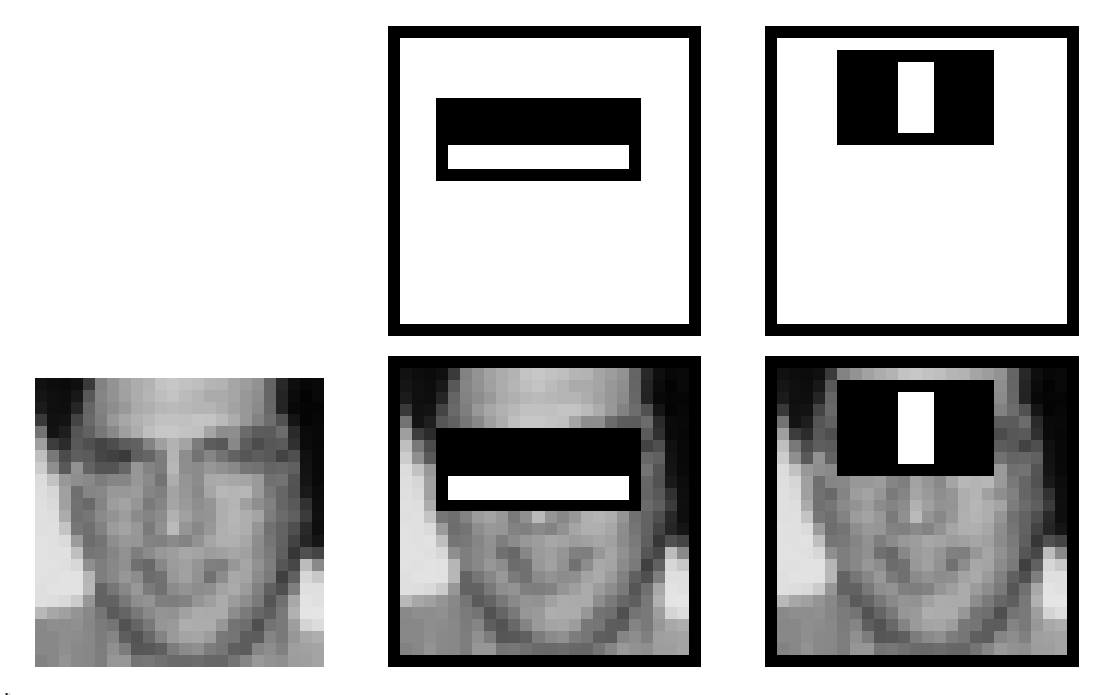
\includegraphics[width=.7\linewidth]{photo_haar.png}
    \caption[Příklad aplikace Haarových příznaků]{Příklad aplikace Haarových příznaků. První měří rozdíl intenzity mezi oblastí očí a líci, druhý porovnává intenzitu v~oblasti očí a nosní přepážky. Obrázek je převzatý~\cite{paperViolaJones}.}
    \label{fig_haar_feature_2}
\end{figure}

Každý příznak je spjat se specifickou oblastí ve vyříznutém okně (částí snímku). Hodnota příznaku se spočítá jako rozdíl součtu intenzity pixelů pod černými a bílými částmi, viz následující rovnice.

\begin{equation}
    \textrm{Value} = \sum (\textrm{pixels in black area}) - \sum (\textrm{pixels in white area})
    \label{eq_haar_feature}
\end{equation}

Je zřejmé, že i pro relativně malý obrázek bude spočítáno velké množství Haarových příznaků. Vzhledem k~tomu, že algoritmus vyžaduje iterovat přes všechny příznaky, musí být spočítány efektivně. Z~tohoto důvodu Viola a Jones navrhli postup, kdy je původní obraz převeden do integrálního obrazu (\textit{integral image}). Jedná se o~způsob reprezentace obrazu tak, že každý bod představuje součet hodnot předchozích pixelů doleva a nahoru, tedy pravý spodní bod obsahuje součet všech pixelů původního obrázku. Reprezentovat obraz tímto způsobem je velmi výhodné, jelikož při počítání intenzity v~segmentu obrazu lze pracovat pouze s~jeho čtyřmi okrajovými body a není nutné procházet všechny pixely v~dané oblasti.

\begin{figure}[H]
    \centering
    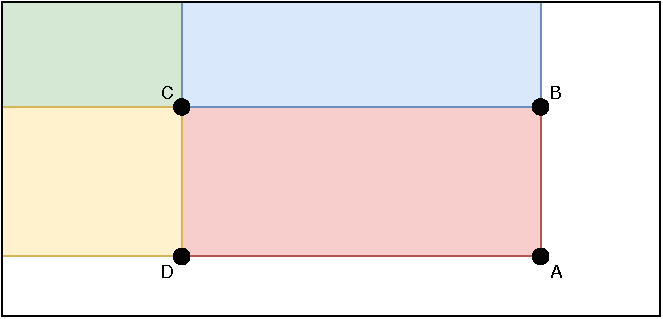
\includegraphics[width=.7\linewidth]{integral-image.pdf}
    \caption[Výpočet plochy na základě integrálního obrazu]{Příklad výpočtu plochy na základě integrálního obrazu. $\textrm{Red area} = A - B - D + C$.}
    \label{fig_integral_image}
\end{figure}

%-------------------------------------------------------------------------------

\subsection*{Histogramy orientovaných gradientů (HOG)}

Koncept rozpoznávání obrazu pomocí techniky histogramů orientovaných gradientů byl znám již od druhé poloviny 80.~let 20.~století. Do širšího povědomí se však algoritmus dostal až v~roce~2005, kdy ho Navneet Dalal a Bill Triggs použili pro detekci chodců ve statických obrázcích ve své práci \textit{Histograms of Oriented Gradients for Human Detection}~\cite{paperDalalTriggs}. Dosahovali výrazně lepších výsledků než do té doby dostupná řešení. Později detektor rozšířili i pro použití ve videu a detekci dalších objektů (aut, zvířat). V~současnosti je HOG detektor implementován v~běžně dostupných knihovnách pro počítačové vidění, např. OpenCV.

Základní myšlenka algoritmu spočívá v~porovnávání, jak je určitá část obrazu tmavá v~porovnání s~částmi, které ji obklopují. V~prvním kroku je možné využít předzpracování pomocí normalizace kontrastu a barev. Dalal a Triggs ale ve své práci demonstrovali, že předzpracování přináší jen velmi malé zpřesnění výsledků, proto je u~mnoha implementací úplně vynecháváno.

Po případném předzpracováním je pro každý pixel ve snímku spočítáno, který pixel kolem něho je nejtmavší. Následně je pixel nahrazen orientovaným gradientem (šipkou), který míří směrem k~nejtmavšímu sousedovi. Gradienty nám tak ukazují tok světla napříč celým obrázkem. Z~původní reprezentace snímku (matice pixelů) dostáváme matici orientovaných gradientů. U~barevných fotografií je gradient vypočten zvlášť pro každý kanál a pro daný pixel je zvolen ten s~nejvyšší hodnotou.

\begin{figure}[H]
    \centering
    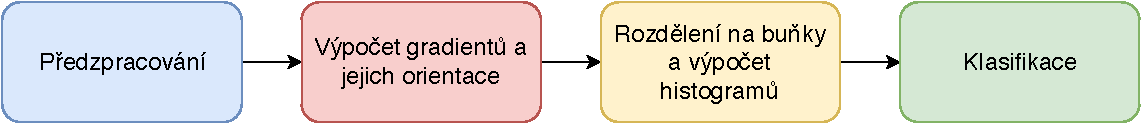
\includegraphics[width=.95\linewidth]{hog-pipeline.pdf}
    \caption[Schéma algoritmu HOG]{Schéma celého algoritmu, který představili Dalal a Triggs.}
    \label{fig_hog}
\end{figure}

Ve druhém kroku je obraz rozdělen na buňky (malé čtverce) $16\times16$~pixelů. Pro každou buňku je spočítán histogram orientovaných gradientů, a tím je zjištěn jejich převažující směr~--~dominantní tok světla v~buňce. Celá buňka je následně nahrazena převažujícím gradientem.

Tímto způsobem je původní obrázek převeden do poměrně jednoduché reprezentace, která však neztratí informaci o~toku světla ve snímku. V~tomto formátu probíhá klasifikace, tedy porovnávání zachycených objektů se vzory a jejich následné zařazení do rozpoznávaných tříd. Algoritmus využívá lineární klasifikátor SVM (Support Vector Machine). Reprezentace histogramy orientovaných gradientů také například dokáže velmi dobře zachytit základní rysy obličeje.

\begin{figure}[H]
    \centering
    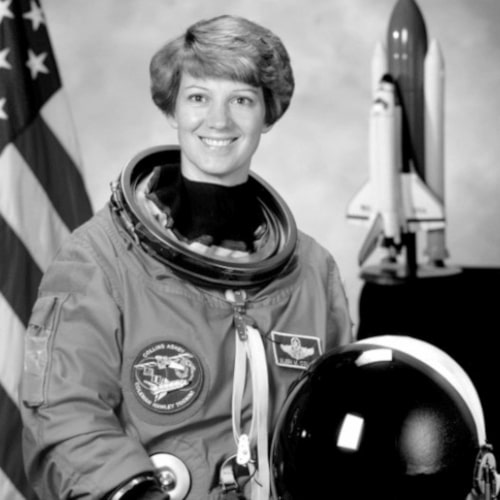
\includegraphics[width=.48\linewidth]{hog_before.jpg}
    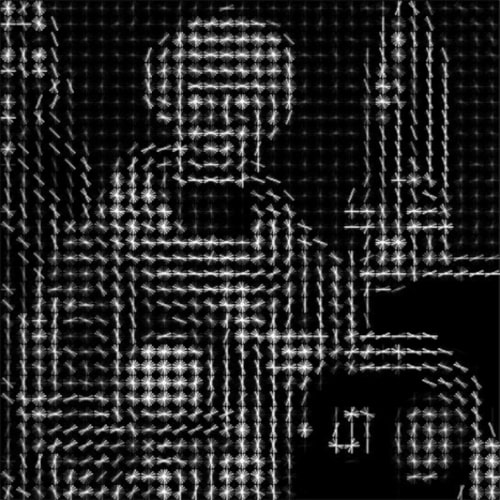
\includegraphics[width=.48\linewidth]{hog_after.jpg}
    \caption[Reprezentace snímku histogramy orientovaných gradientů]{Reprezentace snímku histogramy orientovaných gradientů. Obrázek je převzatý~\cite{docsScikitHog}.}
    \label{fig_hog}
    % Image in full resolution - https://twitter.com/alexjc/status/798113825937625089
\end{figure}

%===============================================================================

\section{Neuronové sítě}
\label{sec_neural_networks}

Neuronové sítě jsou jedním z~výpočetních modelů používaných v~umělé inteligenci. Jeden z~průkopníků neuronových sítí, Dr. Robert Hecht-Nielsen, definuje neuronovou síť jako:

\begin{quote}
    \uv{Počítačový systém tvořený řadou jednoduchých, vysoce propojených procesních prvků, které zpracovávají informace svou dynamickou reakcí na externí vstupy.}~\cite{tdsNeuralNetworks}
\end{quote}

Díky značnému vývoji výpočetního výkonu počítačů a zároveň dostupnosti velkého množství dat, začaly neuronové sítě dosahovat v~oblasti umělé inteligence výsledků, které byly před pár lety ještě nepředstavitelné. Momentálně nabízejí nejlepší řešení v~řadě oblastí umělé inteligence, zejména pak v~oboru zpracování obrazu a rozpoznávání lidské řeči.

Nápad algoritmu založeném na biologickém neurononu vznikl už ve 40.~letech 20.~století. V~70. a 80.~letech byly snahy nápad zrealizovat, ale výpočetní technologie byly absolutně nedostačující pro jakékoliv trénování neuronových sítí~\cite{wikiNeuralNework}. Další výzkum tedy musel počkat na vyšší výpočetní výkon. Během toho byla vymyšlena komplexnější architektura neuronových sítí včetně zpětné propagace, sekce~\ref{sec_multilayer_networks}, a konvolučních vrstev, sekce~\ref{sec_conv_networks}.

První opravdové úspěchy neuronových sítí přišly v~rozpoznávání ručně psaných číslic v~90.~letech, o~to se postaral Yann LeCun~\cite{paperYannLeCun}.

V~roce~2006 přišel Geoff Hilton s~algoritmem pro výrazně rychlejší učení hlubokých neuronových sítí~\cite{paperHilton}. Později ukázal, že pro rozpoznávání lidského hlasu dokáže vytrénovat neuronovou síť v~rámci týdnů.

V~roce~2012 v~soutěži ImageNet Large Scale Visual Recognition (ILSVR), což je soutěž, kde vědci srovnávají výkonnost svých algoritmů, Alex Krizhevsky se svojí konvoluční neuronovou sítí dosáhl suverénně nejlepších výsledků~\cite{paperKriz}.

Na neuronovou síť, přesněji umělou neuronovou síť, se můžeme dívat také jako na výpočetní model inspirovaný biologickou neuronovou sítí, konkrétně zpracováním informací v~lidském mozku.

%-------------------------------------------------------------------------------

\subsection*{Biologická inspirace}

Základní výpočetní jednotkou mozku je neuron. Jedná se o~živou buňku, která je zaměřená na sběr, zpracování a přenos informací. V~lidském nervovém systému se nachází kolem 86~miliard neuronů~\cite{tdsNeuralNetworks}. Každý z~nich má v~průměru 10~tisíc spojů s~jinými neurony. Neuron se skládá z~těla (\textit{cell body}), do kterého přicházejí informace ze vstupních větví -- dendritů (\textit{dendrites}). Výstupní signál, který závisí na vstupech, je dále propagován axonem. Ten je na svém konci mnohačetně rozvětven. Propojení neuronů je uskutečněno pomocí speciálních výběžků -- synapsí. Ty jsou napojeny na dendrity nebo přímo na těla jiných neuronů.

\begin{figure}[H]
    \centering
    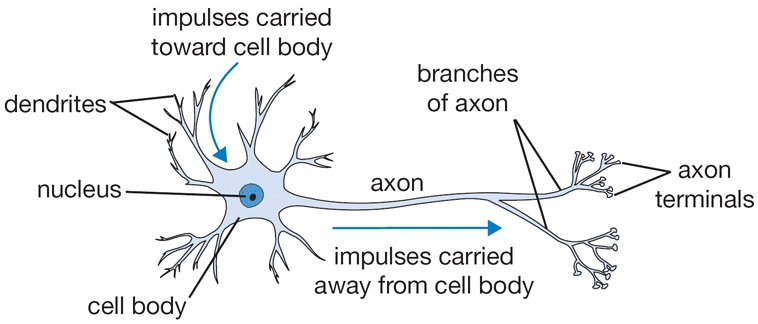
\includegraphics[width=.75\linewidth]{human_neuron.png}
    \caption[Stavba biologického neuronu]{Stavba biologického neuronu. Vstupní informace jsou ze synapsí přijímány dendrity, které impulsy propagují dále do jádra neuronu. Případná reakce neuronu na vstupní podněty je pak přenášena axonem do synapsí a následně buď na dendrit dalšího neuronu, nebo na neuronem ovládanou svalovou buňku. Obrázek je převzatý~\cite{tdsNeuralNetworks}.}
\end{figure}

%-------------------------------------------------------------------------------

\subsection*{Matematický model neuronu}

Základní jednotka matematického modelu neuronové sítě je získána přeformulováním zjednodušené funkce biologického neuronu do matematického jazyka. Tato základní jednotka, matematický neuron, je někdy nazývána jako perceptron. Ilustrace matematického modelu neuronu je zachycena na obrázku~\ref{fig_perceptron}.

Vstup neuronu je získáván z~výstupu jiných neuronů, či externího zdroje. Každému vstupu je přiřazen váhový koeficient, který určuje důležitost vstupu v~porovnání s~ostatními~\cite{haykinNeuralNetworks}. Výstup je vypočítán pomocí tzv. váženého součtu. Jedná se o~součet veškerých hodnot vstupů v~závislosti na jejich váhovém koeficientu. S~výsledkem pak pracuje aktivační funkce (o~nich více v~sekci~\ref{sec_multilayer_networks}), která určí výstup neuronu, viz následující rovnice.

\begin{equation}
    y=f(b + \sum_{i = 1}^{n} w_i x_i)
\end{equation}

Aktivační funkce je značena $f$, vstupy neuronu jako $x$, váhy vstupů $w$ (\textit{weigh}) a $b$ je značeno zkreslení (\textit{bias}). Výstupní hodnota neuronu je označena $y$.

Myšlenka váhových koeficientů je učenlivost, kontrola míry závislosti jednoho neuronu na jiném. Koeficient může nabývat jak pozitivních, tak negativních hodnot. Jestliže je výsledný součet vyšší než prahová hodnota, je neuron probuzen a indikuje signál na svém výstupu ve formě aktivační funkce (též přenosové funkce).

\begin{figure}[H]
    \centering
    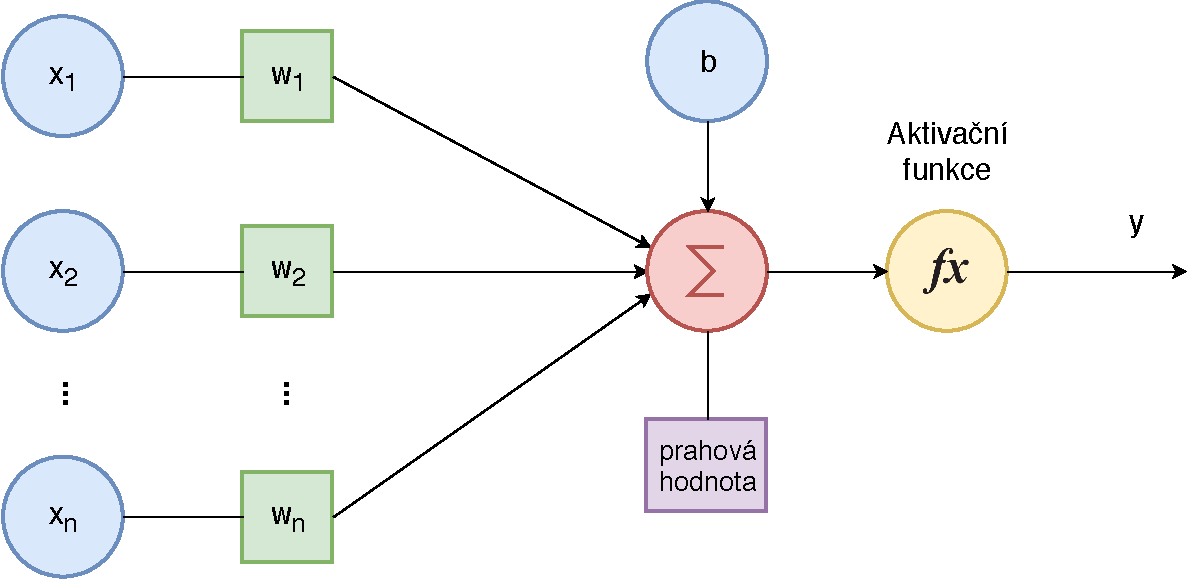
\includegraphics[width=.9\linewidth]{perceptron.pdf}
    \caption[Matematický model neuronu (perceptron)]{Matematický model neuronu (perceptron). Vstupy jsou značeny $x$, jejich váhy $w$ (\textit{weigh}), zkreslení $b$ (\textit{bias}) a výstup $y$. Vše s~příslušnými indexy.}
    \label{fig_perceptron}
\end{figure}

%===============================================================================

\section{Učení neuronových sítí}
\label{sec_training_neural_network}

Cílem učení (trénování) neuronových sítí je nastavit je tak, aby poskytovaly co nejpřesnější výsledky. V~biologických sítích jsou zkušenosti uloženy v~dendritech. V~umělých neuronových sítích jsou zkušenosti uloženy v~jejich matematickém ekvivalentu -- váhách. V~průběhu trénování se tak váhové koeficienty postupně mění a to takovým způsobem, aby nakonec poskytovaly správné hodnoty výstupního signálu na dané vstupní signály. Množina dat, na kterých se síť učí, se nazývá dataset. Po procesu naučení neuronové sítě lze na síť pohlížet jako na černou skříňku (\textit{black box}), která je vhodná k~nasazení ve zvolených aplikačních rovinách~\cite{mendeluNeuralNetworks}.

%-------------------------------------------------------------------------------

\subsection*{Strategie učení}

\textbf{Učení s~učitelem} (\textit{supervised learning}) je strategie, kdy je využíváno zpětné vazby. Neuronové síti je předložen vzor a na základě aktuálních hodnot váhových koeficientů je vypočítán výsledek. Ten je porovnán s~očekávaným výsledkem a následně je spočítána chyba~--~jak moc se aktuálně vypočítaný výsledek neuronovou sítí liší od toho očekávaného. Je-li chyba vyšší než stanovená minimální hranice, je spočítána korekce a jsou upraveny hodnoty vah tak, aby hodnota chyby byla snížena. Toto je opakováno až do dosažení požadované minimální hranice chyby. Poté je síť považována za adaptovanou (naučenou)~\cite{haykinNeuralNetworks}. Při rozpoznávání objektů v~obraze je typické použití strategie učení s~učitelem, kdy se síť učí na předem označených (anotovaných) datech.

\textbf{Učení bez učitele} (\textit{unsupervised learning}) na rozdíl od učení s~učitelem s~výstupem vůbec nepracuje. Neuronové síti jsou postupně předkládány vstupní data bez požadovaných výstupů. Síť je donucena si sama hledat relevantní příznaky, pomocí kterých dokáže data sama roztřídit do skupin. To vede ke shlukování (\textit{clustering}) vstupních dat. Síť se tak naučí reagovat na typického zástupce shluku. Váhy sítě se nastavují tak, aby výstup byl konzistentní, tedy aby síť poskytovala stejnou odezvu na budící signál při stejných nebo podobných vektorech vstupu~\cite{haykinNeuralNetworks}.

%-------------------------------------------------------------------------------

\subsection*{Chybové funkce}

Pro proces učení neuronové sítě je nutný algoritmus, který provádí změnu vah vstupů a výši zkreslení. Obecně až do takové fáze, kdy při vstupu dat z~datasetu výstup odpovídá očekávanému výsledku. Ke zjištění toho, do jaké míry se výstup sítě liší od očekávaného výsledku, se využívá chybových funkcí. Z~jejich výstupu je určeno, jakým směrem a zhruba o~kolik je nutné změnit váhové koeficienty jednotlivých vstupů. Správný průběh učení neuronové sítě lze pozorovat z~hodnot chybové funkce. Ty by se měly každou iteraci snižovat a síť by tak měla lépe aproximovat funkci specifickou pro daný úkol.

\textbf{Mean squared error} (MSE) je základní funkce pro výpočet chyby. Je definována rovnicí~\ref{eq_mse}. $\hat{Y}$ je vektor predikcí, $Y$ je vektor očekávaných výsledků, $n$ velikost těchto vektorů~\cite{bookMse}. Díky umocnění se odstraní záporné hodnoty a dojde ke zvýraznění větších chyb.

\begin{equation}
    \mathrm{MSE}=\frac{1}{n} \sum_{i = 1}^{n} (Y_i - \hat{Y}_i)^2
    \label{eq_mse}
\end{equation}

\textbf{Cross entropy loss} (CE) je chybová funkce definována rovnicí~\ref{eq_ce}. $x$ značí vstupní vektor o~velikosti $N$, $y(x_n, w)$ je výstup z~neuronové sítě za použití vah $w$ a $t_n$ je očekávaný výstup. Funkce se využívá v~případech, kdy výstup může nabývat hodnot z~několika tříd, které nejsou vzájemně výlučné. V~praxi se může jednat například o~rozpoznání objektu v~obraze~\cite{articleCe}.

\begin{equation}
    \mathrm{CE}=\sum_{n = 1}^{N} \sum_{k = 1}^{K} t_{n,k}\mathrm{ln}(y(x_n, w))
    \label{eq_ce}
\end{equation}

%-------------------------------------------------------------------------------

\subsection*{Inicializace vah}

Za inicializaci vah se považuje proces před samotným učením neuronové sítě, kdy se váhám vstupů přiřadí počáteční hodnoty. Správné počáteční hodnoty mohou proces trénování sítě velmi urychlit~\cite{hackernoonXavier}.

Úplně nejjednodušší způsob je vygenerování čistě náhodných počátečních hodnot. To z~pochopitelných důvodů nemusí být ideální, proto se standardně využívají chytřejší techniky. Způsob vhodnosti generování se liší od typů aktivačních funkcí daného neuronu. Typicky je vygenerována hodnota na základě Gaussova rozdělení a následně je vynásobena nějakým výrazem.

\subsubsection*{Pro aktivační funkci hyperbolický tangens}
\begin{enumerate}
    \item Je vygenerována náhodná hodnota dle Gaussova rozdělení se středem~0 a odchylkou~1.
    \item Hodnota je vynásobena výrazem $\sqrt{2/n_i}$, kde $n_i$ je počet vstupních jednotek vrstvy, ve které se neuron nachází.
\end{enumerate}

Někdy může dojít k~problémům známým jako \textit{vanishing gradient} nebo \textit{exploding gradient}~\cite{paperGradientProblems}. Omezení těchto problémů řeší například Xavierova inicializace, která zohledňuje i počet výstupů vrstvy~\cite{hackernoonXavier}.

\subsubsection*{Xavierova inicializace pro aktivační funkci hyperbolický tangens}
\begin{enumerate}
    \item Je vygenerována náhodná hodnota dle Gaussova rozdělení se středem~0 a odchylkou~1.
    \item Hodnota je vynásobena výrazem $\sqrt{2/(n_i+n_o)}$, kde $n_i$ je počet vstupních jednotek a $n_o$ počet výstupních jednotek vrstvy, ve které se neuron nachází.
\end{enumerate}

Pro inicializaci vah je možné rovněž použít hodnoty z~již naučené neuronové sítě, která byla vytrénována k~podobným účelům.

%-------------------------------------------------------------------------------

\subsection*{Přetrénování a podtrénování}

Při učení neuronové sítě je běžné, že se model po určitém počtu iterací dostane do stavu, kdy podává velmi přesné výsledky na trénovacích datech (chybová funkce udává velmi nízké hodnoty), ale při použití nových vstupních dat je přesný méně, než tomu bylo u~nižšího počtu iterací trénování. Tento stav se označuje jako \textbf{přetrénování} (\textit{overfitting, overtraining})~\cite{wikiOverfitting}.

Pro ideální natrénování modelu a zabránění přetrénování je dataset běžně rozdělen na dvě části, trénovací a validační. Trénovací část je typicky značně větší a obsahuje trénovací data~--~data na kterých se model učí. Druhá část jsou tzv. validační data. Ta neslouží pro trénování, ale pouze pro hlídání přetrénování. Na jejich základě se s~váhami modelu nehýbe. Po každé epoše\footnote{Epocha -- iterace trénování, během jedné epochy je předložen síti celý dataset.} se spočítá chyba z~validačních dat. Pokud chyba na trénovacích datech klesá, ale chyba na validačních datech roste, znamená to, že se model dostává do stavu přetrénování.

\begin{figure}[H]
    \centering
    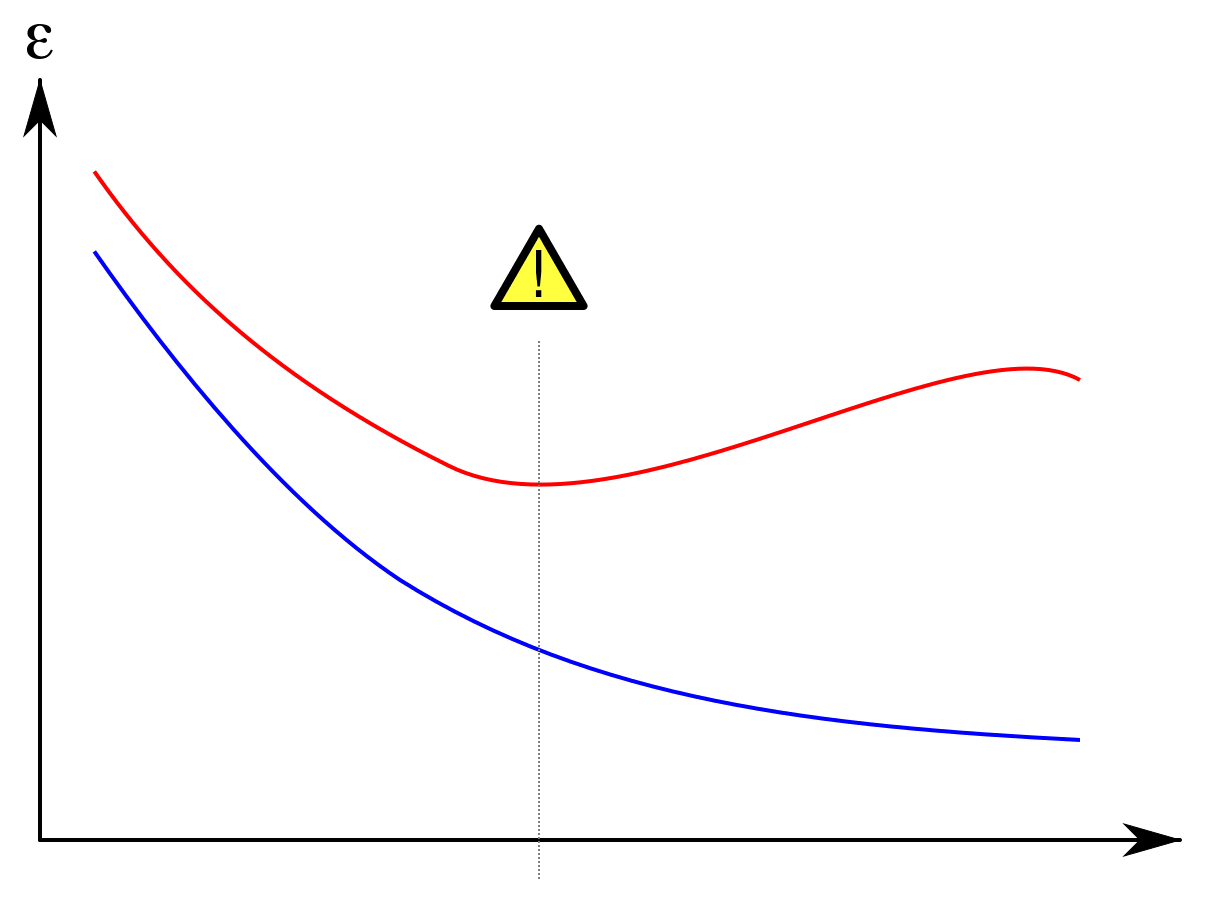
\includegraphics[width=.5\linewidth]{overfitting-1.png}
    \caption[Příznaky přetrénování]{Graf trénovací a validační chyby v~závislosti na počtu odtrénovaných iterací. Trénovací chyba je zakreslena modře, validační chyba červeně. V~momentě, kdy validační chyba začala růst, ale trénovací chyba pokračovala v~klesání, dochází k~přetrénování. Nejideálněji natrénovaný model je po počtu iterací, kdy je validační chyba na svém globálním minumu. Obrázek je převzatý~\cite{wikiOverfitting}.}
    \label{fig_overfitting-1}
\end{figure}

K~přetrénování dochází jelikož množství trénovacích dat je omezené. Model se tak po určité době začne zaměřovat na detaily, které jsou specifické pouze pro danou sadu dat a detektor tak ztrácí na robustnosti, obecnosti (\textit{generalization}). V~extrémním případě si pak model zapamatuje všechna trénovací data a je tak schopen podávat 100\,\%~správné výsledky.

\begin{figure}[H]
    \centering
    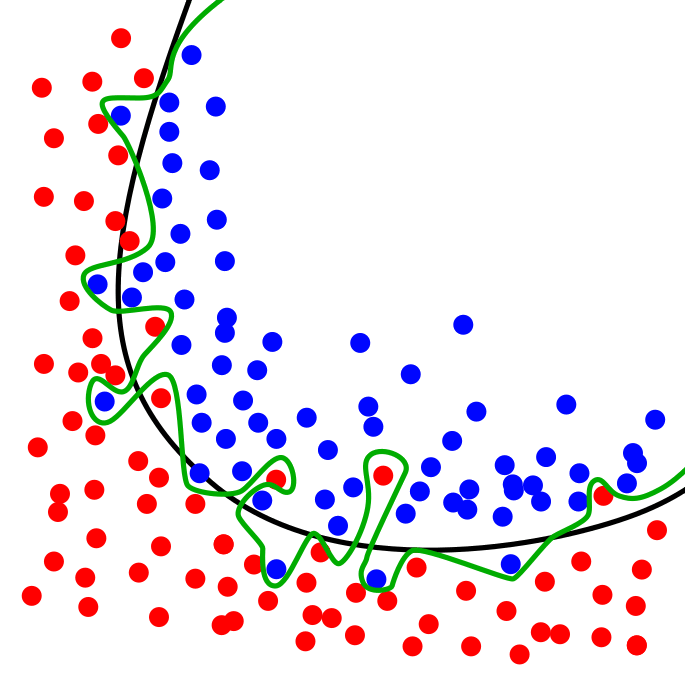
\includegraphics[width=.5\linewidth]{overfitting-2.png}
    \caption[Příklad přetrénovaného klasifikátoru]{Příklad přetrénovaného klasifikátoru na dvou typech dat (červené a modré). Zelená linie reprezentuje přetrénovaný model, černá správně natrénovaný, který dobře aproximuje původní funkci. Zatímco zelená linie perfektně klasifikuje trénovací data, je pro ně příliš uzpůsobená. Je tak pravděpodobné, že při nových datech by podávala vyšší chybovost než klasifikátor černý. Obrázek je převzatý~\cite{wikiOverfitting}.}
    \label{fig_overfitting-2}
\end{figure}

\textbf{Podtrénování} (\textit{underfitting, undertraining}) je jev opačný. Přetrénovaný model dokáže perfektně klasifikovat data, na kterých byl trénován, ale podává špatné výsledky na datech, které nikdy neviděl~\cite{wikiOverfitting}. Podtrénovaný model pak není schopen ani uspokojivě klasifikovat data, na kterých byl trénován a na datech, která nikdy před tím neviděl, pohoří pravděpodobně úplně. Jednoduše chybová funkce je stále vysoká a přesnost modelu nízká.

K~podtrénování dochází, protože model nemůže adekvátně zachytit základní strukturu dat, případně na to neměl dostatek času. Model zkrátka nemusí být vhodný pro naučení se dané struktury. Jedním z~řešení může být úprava modelu. Zvýšení počtu vrstev, zvýšení počtu neuronů, či změnění typů vrstev a jejich přeskládání. Problém ale může být i na straně datasetu, objekt nemusí mít dostatečně specifické příznaky, na základě kterých by ho bylo možné identifikovat.

%===============================================================================

\section{Vícevrstvé neuronové sítě}
\label{sec_multilayer_networks}

Doposud nebylo vysvětleno, jak taková neuronová síť vlastně vypadá. Použití pouze jednoho neuronu není příliš efektivní a dá se využít pouze na velmi jednoduché úlohy (např. klasifikace do dvou tříd)~\cite{mendeluNeuralNetworks}. Ve skutečnosti se setkáváme s~vícevrstvými neuronovými sítěmi (MultiLayer Perceptron -- MLP). Ty jsou tvořeny opakováním základního modelu neuronu, které jsou na sebe napojeny ve vrstvách. Výstup jednoho neuronu je pak vstupem jednoho nebo více neuronů další vrstvy. Způsob propojení neuronů pak určuje architekturu (topologii) sítě.

\begin{figure}[H]
    \centering
    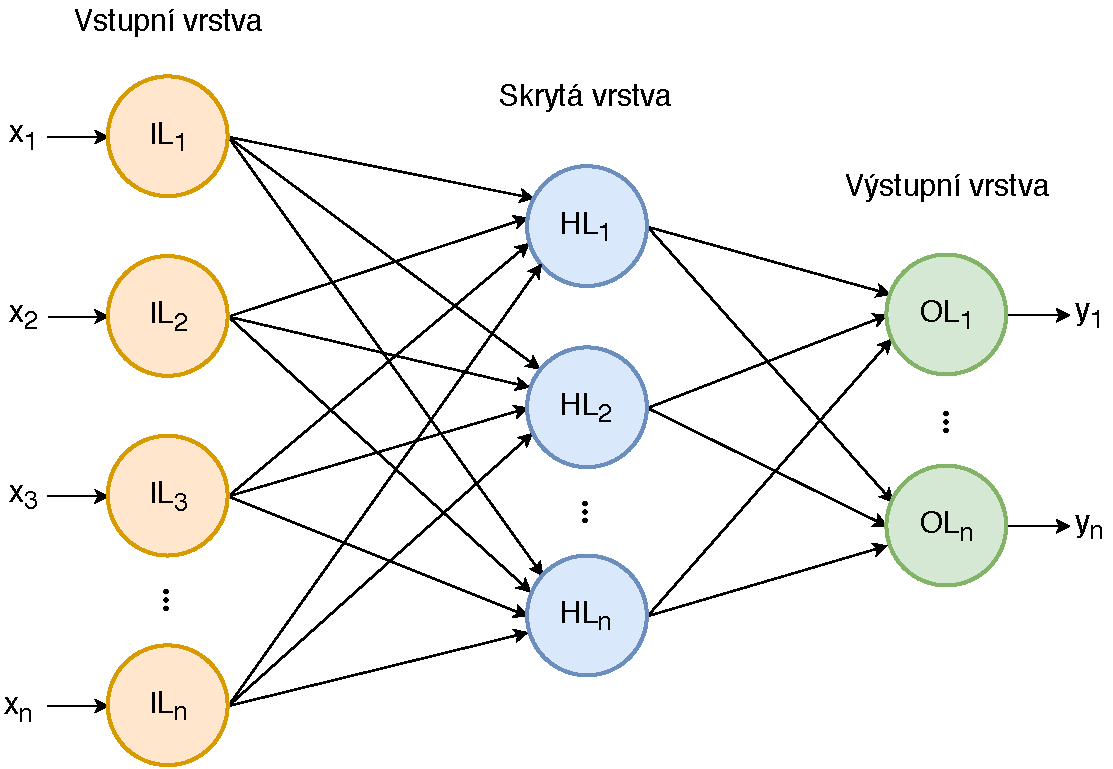
\includegraphics[width=.9\linewidth]{multi_layer.pdf}
    \caption[Architektura vícevrstvé neuronové sítě]{Architektura vícevrstvé neuronové sítě. Síť se skládá z~vrstvy vstupní (\textit{input layer}), skryté (\textit{hidden layer}) a výstupní (\textit{output layer}). Ve vrstvě vstupní neprobíhají žádné výpočty, pouze se propagují externí informace do další vrstvy. Ve vrstvě skryté se informace zpracovávají a poté jsou propagovány do vrstvy výstupní. Ta poskytuje výstup neuronové sítě.}
    \label{fig_multi_layer}
\end{figure}

Počet vstupních neuronů je dán počtem vstupů matematického modelu. Počet neuronů ve skryté vrstvě je volen s~ohledem na složitost úlohy. Čím složitější úloha, tím více neuronů je potřeba pro naučení se potřebných příznaků a pochopení struktury vzoru~\cite{mendeluNeuralNetworks}. Počet výstupních neuronů obvykle odpovídá počtu klasifikačních tříd. Vícevrstvá neuronová síť je standardně učena strategií učení s~učitelem. Neunorová síť může mít více skrytých vrstev, poté o~ní hovoříme jako o~hluboké neuronové síti (Deep Neural Network -- DNN). Jednotlivé skryté vrstvy pak mají různé formy specializace. O~takových sítích mluvíme jako o~konvolučních neuronových sítí a jsou podrobně popsány v~sekci~\ref{sec_conv_networks}. Data, se kterými skryté vrstvy pracují, jsou směrem od vstupu více abstraktní a ke konci sítě lze pomocí příznaků definovat i velmi abstraktní datové struktury. Proces učení se s~robustností sítě stává náročnější.

%-------------------------------------------------------------------------------

\subsection*{Zpětné šíření chyby}

Zpětné šíření chyby (\textit{backpropagation}) je adaptační algoritmus, pomocí kterého lze vypočítat podíl jednotlivých neuronů na celkové chybě sítě a upravit váhy jednotlivých neuronů tak, aby byla minimalizována celková chyba. Jedná se o~nejrozšířenější adaptační algoritmus vícevrtsvých neuronových sítí, je používán přibližně v~80\,\%~všech aplikací neuronových sítí~\cite{ostravaNeuralNetworks}.

Samotný algoritmus se skládá ze tří etap. Nejprve je vstupní signál šířen sítí dopředu (\textit{feedforward}). Ze vstupní vrstvy do vrstev skrytých, kde je spočítán váhový součet všech vstupů a dle aktivační funkce je výstup neuronů směrován do dalších vrstev. Tímto způsobem je signál propagován až do vrstvy výstupní, kde je spočítána celková chyba dle chybové funkce. Dále je chyba šířena neuronovou sítí zpětně od vrstev vyšších k~vrstvám nižším. Každému neuronu je spočítána korekce vah. Ty jsou nakonec aktualizovány a celý proces se opakuje s~dalšími vstupy.

S~konceptem zpětného šíření chyby souvisí problémy \textit{vanishing gradient} a \textit{exploiding gradient}.

%-------------------------------------------------------------------------------

\subsection*{Aktivační funkce}
\label{subsec_activ_function}

Aktivační funkce (také přenosová) slouží pro výpočet výstupní hodnoty neuronu v~závislosti na jeho vektoru vstupních hodnot. Je-li neuron probuzen, aktivační funkce moduluje výstupní signál, ten je směrován do další úrovně neuronové sítě. Bez aktivačních funkcí by výstup neuronu mohla být jakákoliv hodnota od mínus nekonečna až do plus nekonečna. Aktivační funkce poskytuje tedy jisté hranice, mezi kterými může neuron produkovat hodnoty~\cite{mediumActivationFunctions}. Aktivační funkce dávají vědět neuronům další úrovně, zda mají považovat neuron za aktivovaný, nebo ne. Volba aktivační funkce má výrazný vliv na dobu učení (trénování) neuronové sítě. Její výběr je často ovlivněn zkušenostmi z~řešení obdobných úloh, mnohdy je nutné experimentovat.


\textbf{Funkce jednotkového skoku} (také Heavisideova funkce) je nejjednodušší přenosová funkce. Jedná se o~nespojitou funkci, která nabízí pouze dvě možné hodnoty výstupu. $1$,~pokud vážený součet je vyšší nebo roven prahové hodnotě ($t$ -- \textit{treshold}) a $0$,~pokud nikoliv~\cite{mediumActivationFunctions}.

\begin{equation}
    f(x)=\left\{\begin{matrix}
        0 & x < t \\
        1 & x \geq t
    \end{matrix}\right.
\end{equation}

Funkce jednotkového skoku může posloužit jako binární klasifikátor. Při klasifikaci do více tříd by bylo problémové síť tvořenou neurony s~funkcí jednotkového skoku dovést ke konvergenci. V~takovém případě by byla žádoucí funkce, která by dokázala vyjádřit například aktivováno z~20\,\%, ze~70\,\% apod.

\begin{figure}[H]
    \centering
    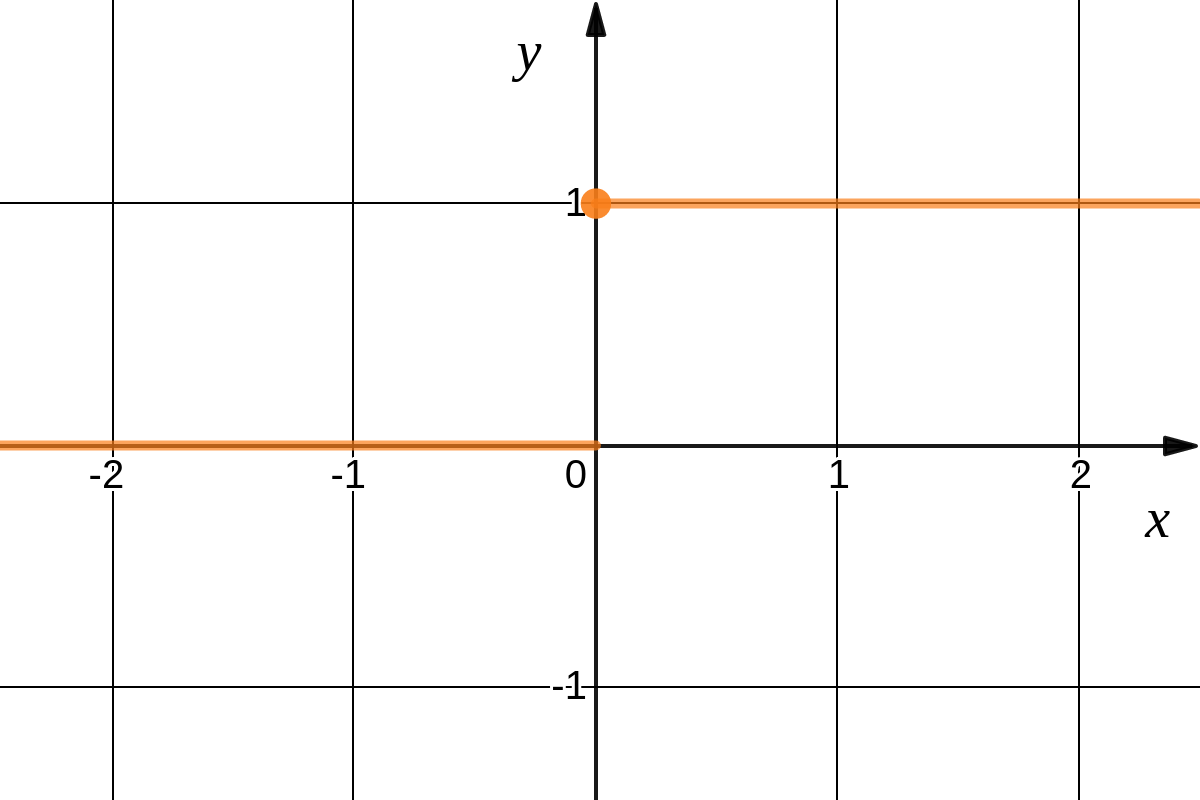
\includegraphics[width=.5\textwidth]{hardlim.png}
    \caption[Graf funkce jednotkového skoku]{Graf funkce jednotkového skoku.}
    \label{fig_hardlim}
\end{figure}


\textbf{Lineární funkce} podává výstup proporcionálně roven vstupům~--~váženému součtu hodnot na vstupu a přičtení zarovnání. Aktivace mohou mít různou sílu, problém jako u~funkce jednotkového skoku tu tak není~\cite{mediumActivationFunctions}.

\begin{equation}
    f(x)=ax
\end{equation}

Problém však nastává při výpočtu gradientního sestupu (\textit{gradient descent}), který slouží pro optimalizaci při trénování. Derivace lineární funkce je totiž konstantní, není nijak závislá na hodnotě vstupu $x$. Pokud nastane chyba v~predikci, změny prováděné zpětnou propagací jsou konstantní a nejsou závislé na změně vstupu $x$.

Toto ovšem není jediný problém. Mějme vícevrstvou neuronovou síť, kde je v~každé vrstvě použita lineární aktivační funkce. První vrstva je aktivována lineární funkcí. Tato aktivace zase vstupuje do další úrovně jako vstup. Další vrstva vypočítává vážený součet a podává výstup opět na základě jiné lineární funkce. To má za následek, že poslední aktivační funkce bude pouze lineární funkcí vstupů první vrstvy a všechny vrstvy by tedy bylo možné nahradit pouze jedinou.

\begin{figure}[H]
    \centering
    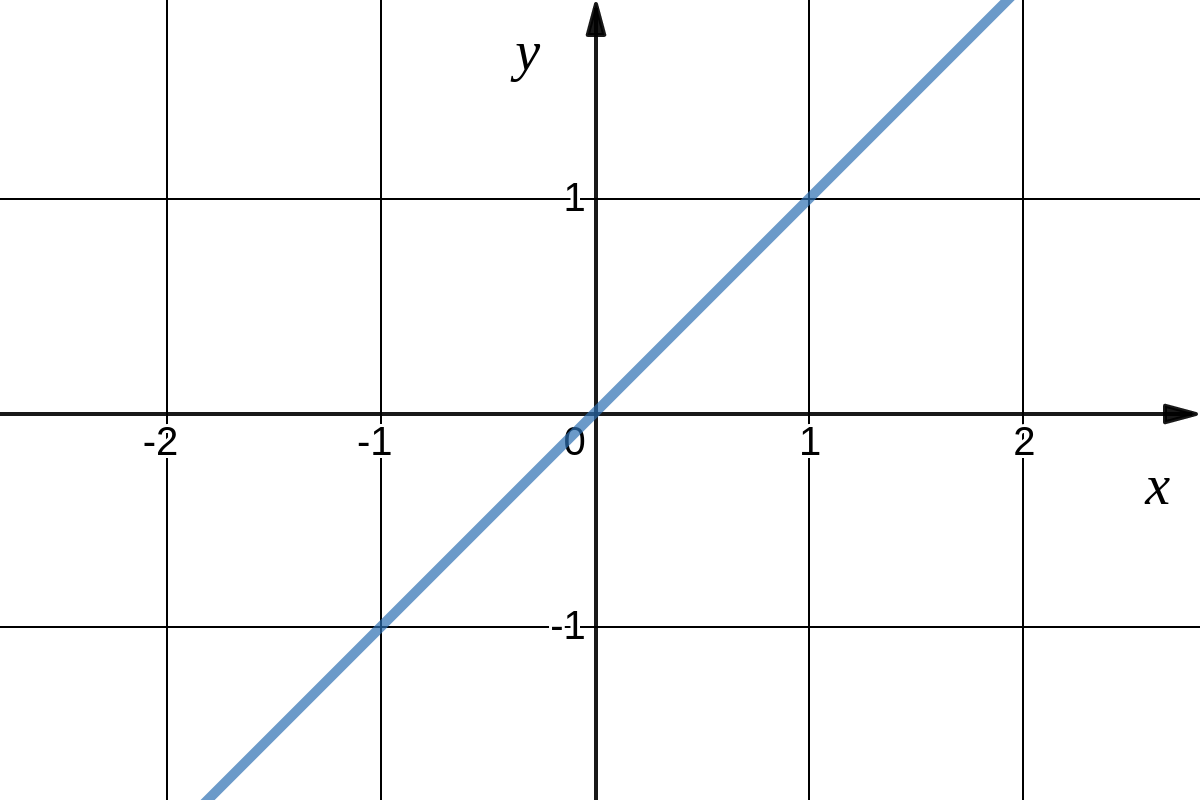
\includegraphics[width=.5\textwidth]{purelin.png}
    \caption[Graf lineární funkce]{Graf lineární funkce.}
    \label{fig_lin}
\end{figure}


\textbf{Sigmoidální přenosová funkce} dává výstupy z~internalu~$(0,1)$. Funkce a její kombinace jsou nelineární. Její derivace je tak závislá na hodnotách vstupů. Problémy s~výpočtem gradientního sestupu jsou pryč a stejně tak je možné efektivně skládat vrstvy neuronů za sebe~\cite{mediumActivationFunctions}.

\begin{equation}
    f(x)=\frac{e^{x}}{e^{x}+1}
\end{equation}

Funkce roste v~intervalu~$(-2, 2)$ velmi strmě. Což znamená, že jakákoliv malá změna vstupů $x$ v~tomto intervalu, má za následek poměrně výraznou změnu na výstupu $y$. To má za následek, že funkce má tendenci vracet hodnoty $y$ blízko hraničním hodnotám. Pokud jsou hodnoty vstupu naopak mimo zmíněný interval, rozdíly ve vrácené hodnotě mohou být velmi malé. To znamená, že síť se v~některých případech nedokáže v~rozumném čase učit. Tento problém je znám jako \textit{vanishing gradient}.

Tyto vlastnosti činí funkci sigmoid oblíbenou a často používanou v~hlubokých neuronových sítích.

\begin{figure}[H]
    \centering
    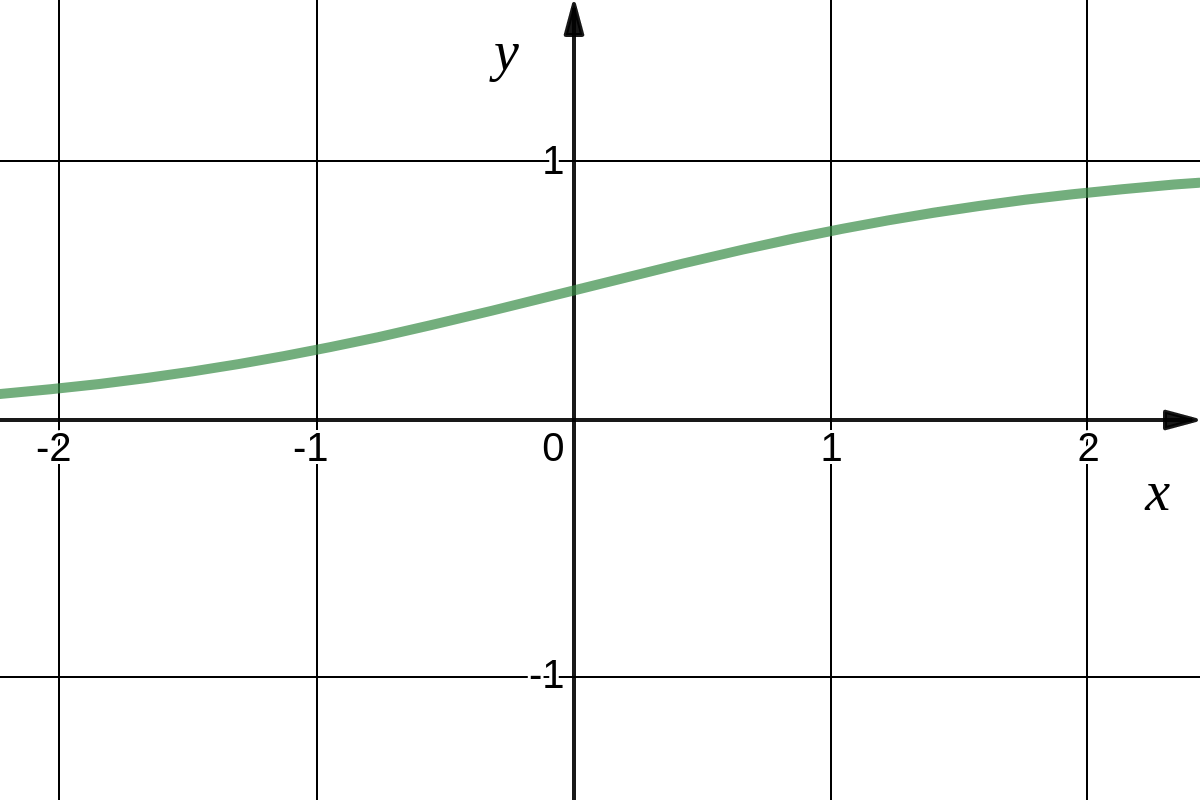
\includegraphics[width=.5\textwidth]{logsig.png}
    \caption[Graf sigmoidální funkce]{Graf sigmoidální funkce.}
    \label{fig_logsig}
\end{figure}


\textbf{Hyperbolický tangens} je hyperbolická funkce definována pomocí hyperbolického sinu a cosinu. Její průběh je podobný jako u~sigmoidní funkce a potýká se se stejnými problémy (\textit{vanishing gradient}). Obor hodnot~$(-1, 1)$ je vycentrovaný okolo nuly, což usnadňuje optimalizace~\cite{mediumActivationFunctions}.

\begin{equation}
    f(x)=\mathrm{tanh}(x)=\frac{e^{2x}-1}{e^{2x}+1}
\end{equation}

Hyperbolický tangens je tak také velmi populární a široce používaná aktivační funkce.

\begin{figure}[H]
    \centering
    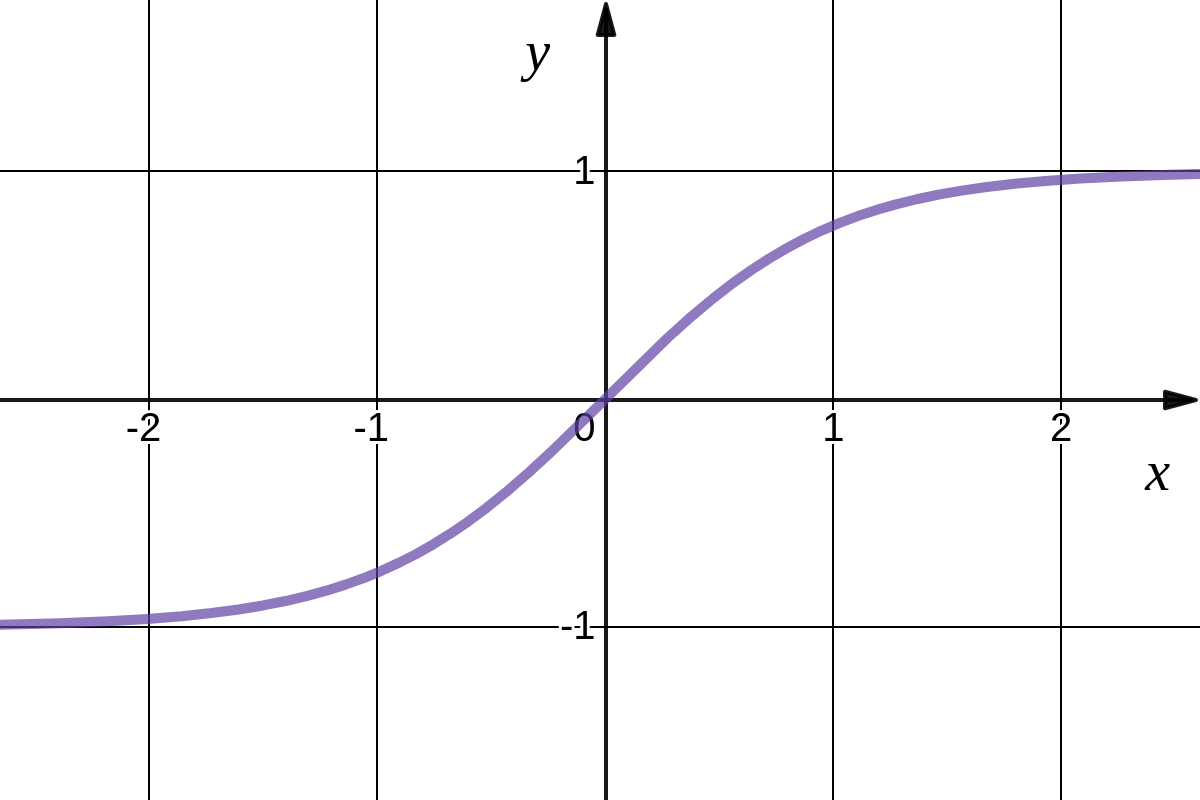
\includegraphics[width=.5\textwidth]{tansig.png}
    \caption[Graf funkce hyperbolický tangens]{Graf funkce hyperbolický tangens.}
    \label{fig_tansig}
\end{figure}


\textbf{Rectified linear unit} (ReLU) je aktivační funkce, která vrací~$0$ pro záporné hodnoty a~$x$ pro hodnoty kladné. Na první pohled se může zdát, že se bude potýkat se stejnými problémy jako lineární funkce. ReLU a její kombinace jsou ale nelineární povahy a ve skutečnosti dokáží dobře aproximovat jakoukoliv funkci~\cite{mediumActivationFunctions}.

\begin{equation}
    f(x)=\left\{\begin{matrix}
        0 & x < 0  \\
        x & x \geq 0
    \end{matrix}\right.
\end{equation}

Díky tomu, že ReLU zahrnuje jednodušší matematické operace, jsou její výpočetní nároky oproti sigmoidní funkci a hyperbolickému tangentu výrazně nižší. Proto je v~umělých neuronových sítí často využívána~\cite{articleNeuralNetworksOverview}.

\begin{figure}[H]
    \centering
    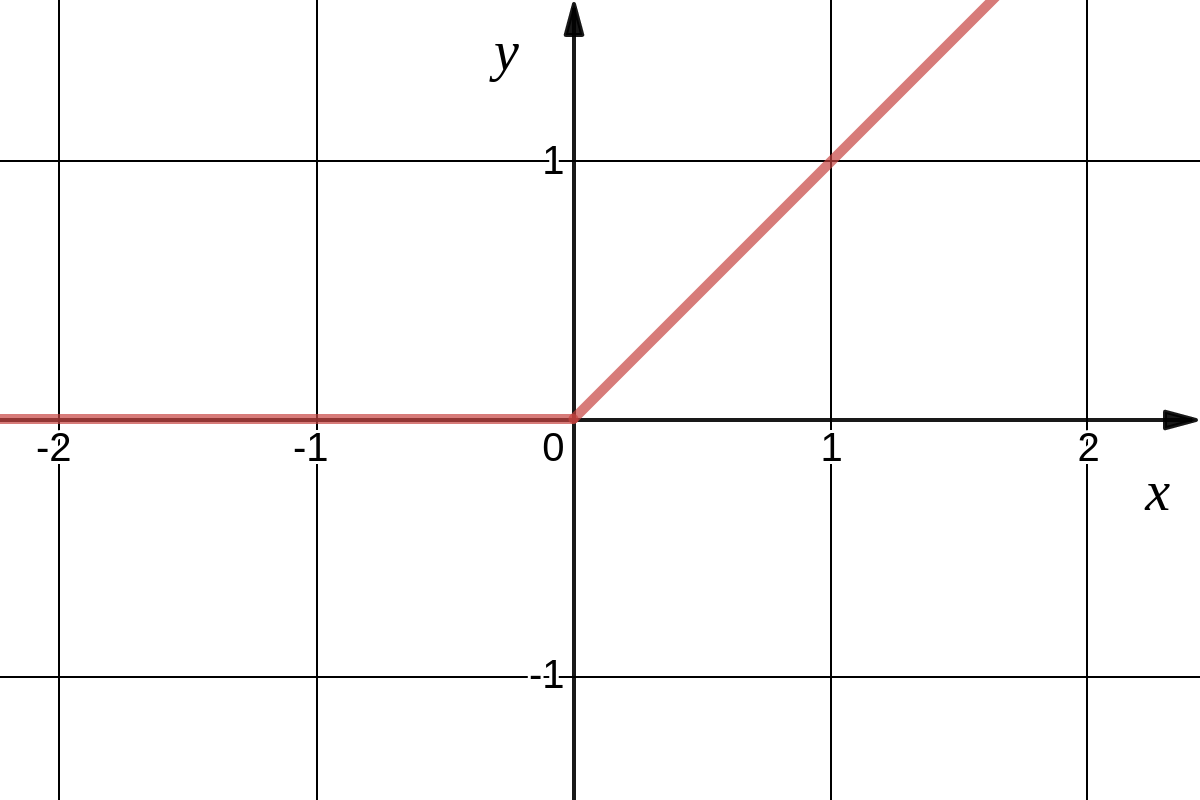
\includegraphics[width=.5\textwidth]{relu.png}
    \caption[Graf funkce ReLU]{Graf funkce ReLU.}
    \label{fig_relu}
\end{figure}


\textbf{Funkce softmax} se využívá v~posledních vrstvách neuronových sítí, zejména u~klasifikačních úloh, například přiřazení objektu do předem definovaných tříd, které nejsou vzájemně výlučné. Funkce je definována následující rovnicí~\cite{mediumActivationFunctions}.

\begin{equation}
    f_i(\vec{x})=\frac{e^{x_i}}{\sum^N_{n=1} e^{x_n}}
\end{equation}

Funkce softmax normalizuje $N$ rozměrný vektor $\vec{x}$ do $N$ rozměrného vektoru $f(\vec{x})$, jehož jednotlivé prvky dávají v~součtu hodnotu 1. Jelikož není možné načrtnout obecnou křivku funkce softmax, je místo grafu uveden příklad s~konkrétními hodnotami na následující rovnici.

\begin{equation}
    f([1; 2; 3; 4; 5])=\frac{[e; e^2; e^3; e^4; e^5]}{e+e^2+e^3+e^4+e^5} = [0,012; 0,032; 0,086; 0,234; 0,636]
    \label{eq_softmax_example}
\end{equation}

%===============================================================================

\section{Konvoluční neuronové sítě}
\label{sec_conv_networks}

Konvoluční neuronové sítě (Convolutional Neural Networks -- CNN) jsou hluboké neuronové sítě, kde jednotlivé skryté vrstvy mají jistou formu zaměření pro konkrétní činnost. Jsou speciálně navrženy pro rozpoznávání dvojrozměrných tvarů s~vysokým stupněm invariance. Jinými slovy, rozpoznávaný objekt může být nějakým způsobem deformován, může být zachycen v~různých rozlišeních či se lišit v~detailech, i přesto by ho konvoluční neuronová síť měla rozpoznat.~\cite{haykinNeuralNetworks} Typy vrstev používané při zpracování obrazu jsou vysvětleny dále.

%-------------------------------------------------------------------------------

\subsection*{Typy vrstev}

\textbf{Plně propojená vrstva} (\textit{fully connected layer} nebo \textit{dense layer}) spojuje každý neuron z~dané vrstvy s~každým neuronem vrstvy následující. Jedná se o~stejný princip jako u~klasických vícevrstvých neuronových sítí, které byly představeny v~sekci~\ref{sec_multilayer_networks}. Ačkoliv jsou sítě s~plně propojenými vrstvami schopny dobře aproximovat libovolnou funkci, jejich vysoký počet spojení výrazně zvyšuje nároky na výpočetní kapacity. Proto se vyskytují spíše až v~koncových vrstvách konvolučních sítí, kde mají na starosti klasifikaci objektů~\cite{bookElementsNeuralNets}.


\textbf{Konvoluční vrstvy} (\textit{convolutional layers}) jsou hlavní stavební kameny konvolučních neuronových sítí. Jejich název je převzat od jména matematické operace, která se ve vrstvě provádí -- konvoluce. Obraz je reprezentován diskrétními hodnotami pixelů, konkrétně maticí těchto hodnot, proto nás bude zajímat diskrétní 2D~konvoluce~\cite{paperLecunNature}. Ta je definována rovnicí~\ref{eq_convolution}.

\begin{equation}
    f(x,y) \star h(x,y)=\sum_{i=-k}^{k}\sum_{j=-k}^{k}f(x-i,y-j)\cdot h(i,j)
    \label{eq_convolution}
\end{equation}

Symbol $\star$ je operátor konvoluce nad funkcemi $f(x,y)$ a $h(x,y)$. První operand, v~našem případě funkce $f$, obvykle značí vstupní obraz a druhý operand, funkce $h$, značí konvoluční jádro (filtr).

\begin{figure}[H]
    \centering
    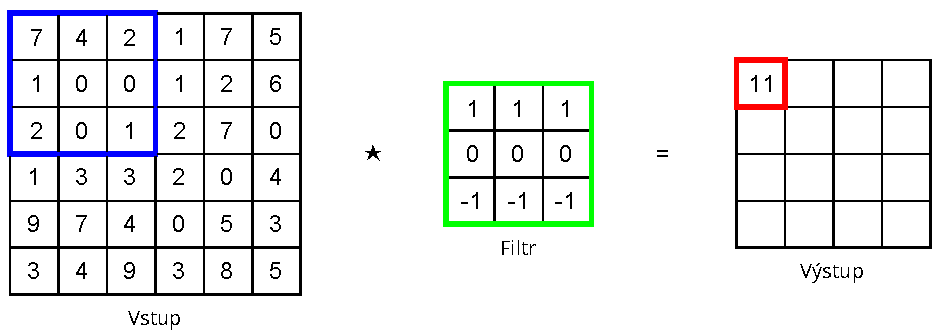
\includegraphics[width=.9\linewidth]{convolution.pdf}
    \caption[Příklad výpočtu konvoluce]{Příklad výpočtu konvoluce. Vstup jsou náhodně vygenerované hodnoty, pro zpracování obrazu by se jednalo o~hodnoty jednotlivých RGB kanálů případně hodnoty jasu. Konvoluční filtr může vypadat například takto, ale může se jednat i o~matici jiné velikosti.}
    \label{fig_conv_ex}
\end{figure}

Výstupní matice je menší než vstupní. To je důsledkem toho, že pro výpočet jednoho výsledného bodu potřebujeme na vstupu matici o~velikosti filtru. Pokud chceme zmenšení rozlišení předejít, dá se původní matice rozšířit. A~to buď nulovými body (\textit{zero padding}), případně
jinými, vhodně vybranými hodnotami.

Parametry konvoluční vrstvy se skládají z~množiny konvolučních filtrů. Samotná síť se učí optimalizací jejich jednotlivých hodnot. Filtry jsou po vstupu posouvány po určitém kroku a je počítána výsledná dvoudimenzionální mapa~\cite{paperLecunNature}. Konvoluční filtry mohou mít různá uplatnění. Například pro rozmazaní či doostření obrazu, ale také pro  detekci hran. Hrana je rozpoznána prudkou změnou světelných podmínek. Podstata filtru je nalézt gradient, tj. směr maximální změny, který hranu charakterizuje~\cite{mendeluDigital}.

Vlivem výpočtu v~konvolučních vrstvách může dojít k~tomu, že některé hodnoty v~matici nabudou záporných hodnot. Barvy jsou ale reprezentovány třemi kanály v~rozmezí~0\,--\,255. Proto je používána přenosová funkce ReLU, viz obrázek~\ref{fig_relu}, která odstraní negativní hodnoty z~aktivační mapy. Dají se použít i jiné funkce, ale ReLU se ukázala jako nejefektivnější~\cite{paperKriz}.


\textbf{Pooling vrstva} je další typický druh vrstvy konvolučních neuronových sítí. \textit{Pooling}, neboli sdružování slouží pro podvzorkování~--~zmenšení rozměrů dvoudimenzionální mapy. Tím se zmenší počet parametrů sítě a dojde ke snížení výpočetních nároků pro další vrstvy. Realizuje se agregací několika sousedních buněk do jedné. Nejběžnější způsoby jsou \textit{average pooling}, kdy se počítá průměrná hodnota z~agregovaných buněk a \textit{max pooling}, kdy se vybírá maximální hodnota~\cite{paperLecunNature}.

\begin{figure}[H]
    \centering
    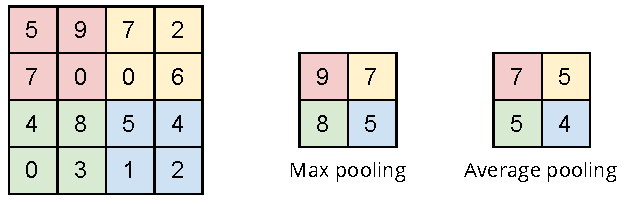
\includegraphics[width=.75\linewidth]{pooling.pdf}
    \caption[Příklad max a averige poolingu]{Příklad \textit{average pooling} a \textit{max pooling} na jednoduché $4 \times 4$~matici do matice o~rozměrech~$2 \times 2$.}
    \label{fig_pooling_ex}
\end{figure}

Za sdružováním stojí myšlenka, že úplně přesná lokace příznaku není pro klasifikaci důležitá. Naopak může být na škodu a podpořit problém přetrénování sítě, viz sekce~\ref{sec_training_neural_network}. Důležitější je tedy relativní lokace příznaku vzhledem k~ostatním. Tím se dosáhne větší obecnosti detektoru (generalizace)~\cite{paperLecunNature}.

Pooling vrstva se běžně vkládá mezi jednotlivé konvoluční vrstvy. V~současnosti se nejvíce používá přístup \textit{max pooling}, který v~praxi funguje nejlépe~\cite{paperPoolingTypes}.


\textbf{Dropout vrstva} má za úkol snížit náchylnost sítě k~přetrénování. Spočívá v~nastavení výstupu každého neuronu ve skryté vrstvě na~0 s~pravděpodobností~50\,\%. K~deaktivaci neuronů dochází u~každého vzorku dat při trénování, do učení je tak uměle přidáván šum, díky kterému je síť schopna více generalizovat. Dropout vrstva zvýšuje počet potřebných iterací k~dosažení konvergence~\cite{paperKriz}.


\textbf{Ztrátová vrstva} (\textit{loss layer}) specifikuje jak proces trénování penalizuje rozdíl mezi predikcí sítě (výstupem) a skutečnými hodnotami (označená trénovací data). Jedná se o~finální vrstvu neuronové sítě. Existuje mnoho chybových funkcí určené pro různé typy úloh, viz sekce~\ref{sec_training_neural_network}.

%-------------------------------------------------------------------------------

\subsection*{Architektura konvolučních neuronových sítí}

Samotných architektur konvolučních neuronových sítí je velké množství. Jednotlivé implementace se od sebe liší typem použitých vrstev a jejich množstvím. Na obrázku~\ref{fig_conv_arch} je příklad napojení jednotlivých vrstev za sebe.

\begin{figure}[H]
    \centering
    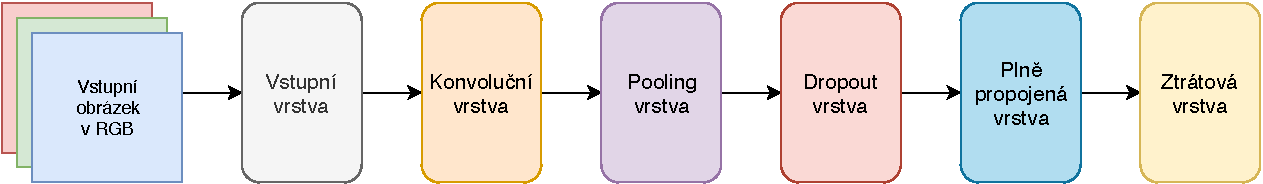
\includegraphics[width=.99\linewidth]{conv-arch.pdf}
    \caption[Ukázka napojení vrstev konvolučních sítí]{Ukázka napojení jednotlivých vrstev za sebe.}
    \label{fig_conv_arch}
\end{figure}

Na samém začátku je vstupní obraz reprezentovaný většinou třemi barevnými kanály. Vstupní vrstva čte hodnoty pixelů a propaguje je do dalších vrstev. V~konvoluční vrstvě probíhá konvoluce. Je jich většinou několik a každá se snaží porozumět jiným základním vzorům. Například první konvoluční vrstva se snaží rozpoznávat hrany, další se snaží porozumět tvaru, barvě apod. Během procesu učení se mění hodnoty buněk jednotlivých filtrů. Konvoluční vrstvy obsahují přechodovou funkci ReLU pro odstranění případných záporných hodnot. Pooling vrstva provede podvzorkování pro dosáhnutí větší generalizace a snížení výpočetních nároků. Dropout vrstva zabraňuje přetrénování. Výstupy z~některých neuronů nejsou použity, tím se do sítě zanese uměle vytvořený šum. Síť tak nebude tolik závislá na trénovacím datasetu, ale bude fungovat obecněji. Plně propojená vrstva provádí klasifikaci, typicky jich také bývá více. Při učení nastavujeme váhy pro každý vstup každého neuronu. Ztrátová vrstva dává zpětnou vazbu, jak moc se výsledek sítě liší od označených trénovacích dat.

%===============================================================================

\section{Detekční sítě}
\label{sec_detection_networks}

Doposud bylo představeno využití neuronových sítí pouze pro klasifikaci obrazu. Předpokládalo se, že na snímku je pouze jeden dominantní objekt, který bude porovnáván se známými vzory a bude vyhodnocena jejich vzájemná podobnost. V~reálném světě se ale ve snímcích vyskytuje velká spousta různých objektů odlišných velikostí. Je nutné zajistit nějaký mechanismus, který rozpozná, že se jedná o~objekt hodný klasifikace. Obraz kolem něho ořízne a danou výseč předá klasifikátoru, který následně rozhodne, kam objekt zařadit.

\begin{figure}[H]
    \centering
    
\includegraphics[width=.49\textwidth]{cat.jpg}\hfill
    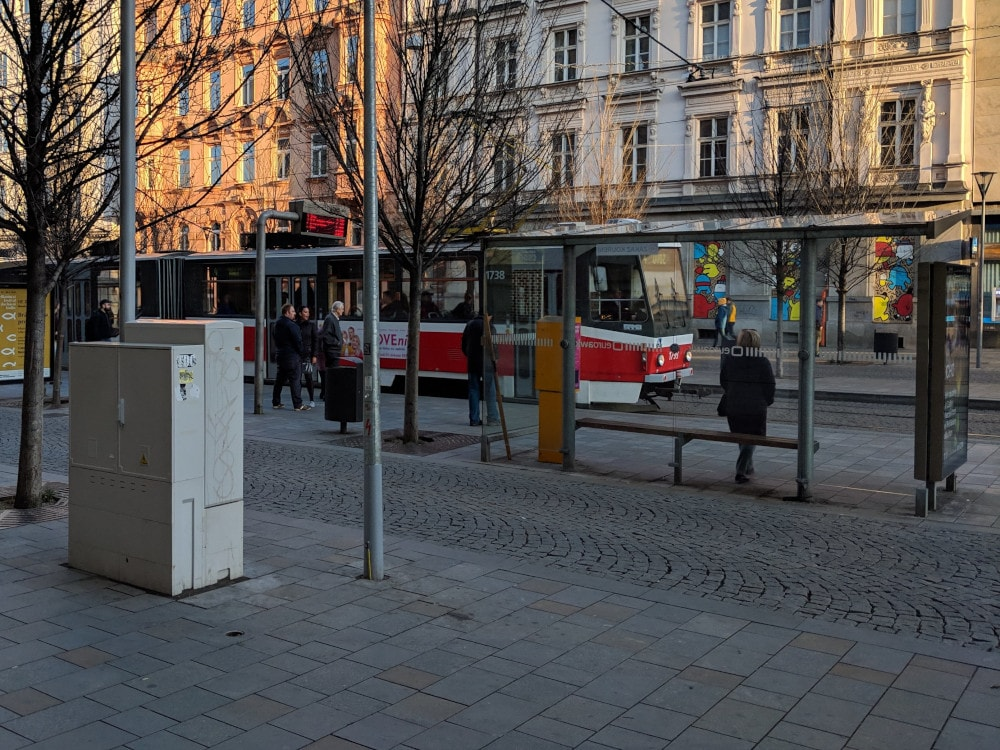
\includegraphics[width=.49\textwidth]{street.jpg}
    \caption[Motivace k~algoritmům detekce objektů]{Na levé straně je obrázek kočky. Na snímku je zachycen a perfektně oříznut pouze jeden objekt. To z~obrázku dělá ideální snímek pro klasifikaci. Na pravé straně je pro změnu fotka ulice, kde se nachází spousta objektů, s~různým pozadím a různě se navzájem překrývajících.}
    \label{fig_cat_street}
\end{figure}

Naivní algoritmus detekce objektů by mohl spočívat v~posouvání různě velikých oken po obraze a následné výseče předávat nějaké konvoluční neuronové síti, která by segment klasifikovala. Toto je velmi silový (\textit{brute force}) způsob, který by byl velmi výpočetně náročný a neefektivní. Existují lepší řešení, které dokáží vybírat podezřelé oblasti z~obrazu a ty poté předávat klasifikátoru.

Rozlišujeme detektory jednostupňové (\textit{one-stage}) a dvoustupňové (\textit{two-stage}). První jmenované zvládají detekci i klasifikaci v~jednom kroku, jsou typicky rychlejší, ale méně přesné. Dvoustupňové pak rozdělují proces detekce a klasifikace zvlášť~--~obraz se musí zpracovávat dvakrát. To má za následek pomalejší celkové zpracování, ale větší přesnost (10\,--\,40\,\%)~\cite{paperFocalLoss}.

%-------------------------------------------------------------------------------

\subsection*{R-CNN}

R-CNN (Region-based Convolutional Neural Network) a další detektory z~něj vycházející byly významným pokrokem v~oblasti detekce objektů. Jedná se o~dvoustupňový detektor~\cite{mediumRcnn}.

Nejprve je využit algoritmus pro detekci podezřelých oblastí (\textit{region proposals}) nezávisle na tom, do jaké kategorie by objekt mohl spadat. Jedná se o~algoritmus selektivního vyhledávání, který prochází zdrojový obraz a snaží se spojit pixely stejné nebo podobné barvy~\cite{paperRcnn}. U~nich lze předpokládat, že náleží jednomu objektu.

\begin{figure}[H]
    \begin{tabular}{cc}
        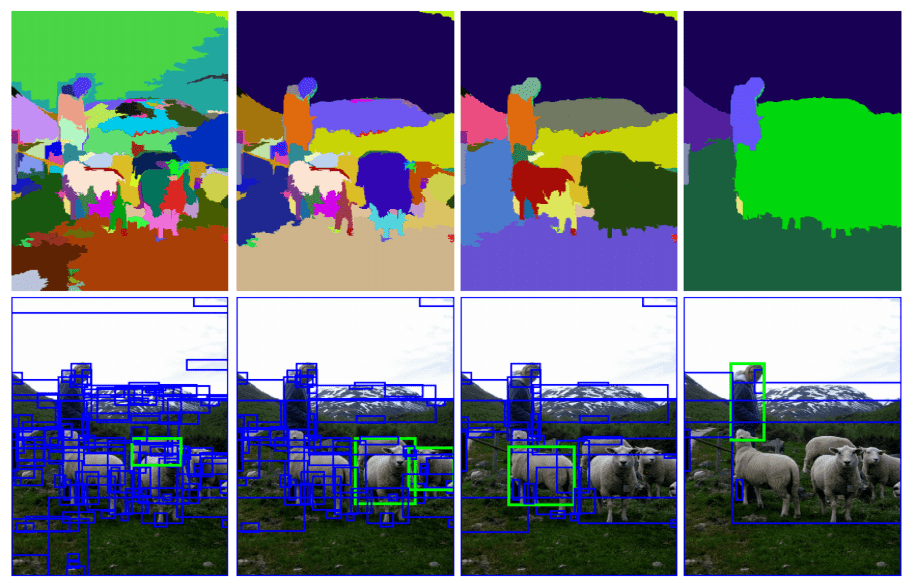
\includegraphics[width=.49\textwidth]{selective_search-1.png}\hfill
        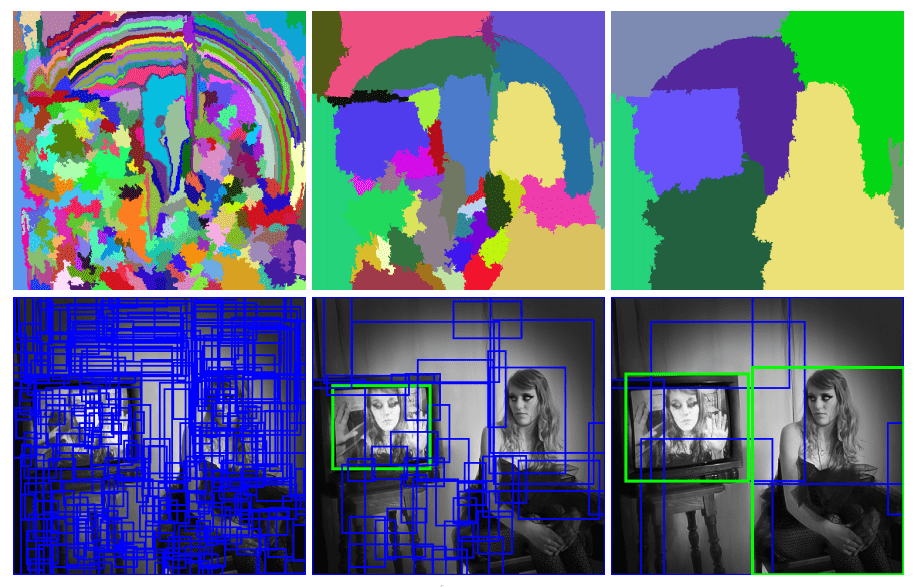
\includegraphics[width=.49\textwidth]{selective_search-2.png}
    \end{tabular}
    \caption[Ukázky selektivního vyhledávání detektoru R-CNN]{Dvě ukázky selektivního vyhledávání a jeho práci s~rozdílnými měřítkami pro spojování barevných pixelů. Obrázky jsou převzaté~\cite{mediumRcnn}.}
    \label{fig_selective_search}
\end{figure}

Těchto výsečí je nalezeno kolem~2000. Po nalezení jsou zdeformovány a předány konvoluční neuronové síti (AlexNet~\cite{paperKriz}). Ta provede výpočet příznaků, na základě kterých pak klasifikátor SVM (Support Vector Machine) rozhodne, zda se skutečně jedná o~objekt a jaké třídě s~jakou pravděpodobností náleží~\cite{paperRcnn}.

Původní model nebyl dostatečně rychlý především kvůli rozdělení celého procesu do několika postupných fází (regrese ohraničení, extrakce příznaků pomocí konvoluční sítě a klasifikace pomocí SVM). Pro každý snímek musela konvoluční síť AlexNet spočítat příznaky pro 2000~výsečí. Z~tohoto důvodu přišlo několik dalších detektorů, které původní R-CNN zdokonalily.

\begin{figure}[H]
    \centering
    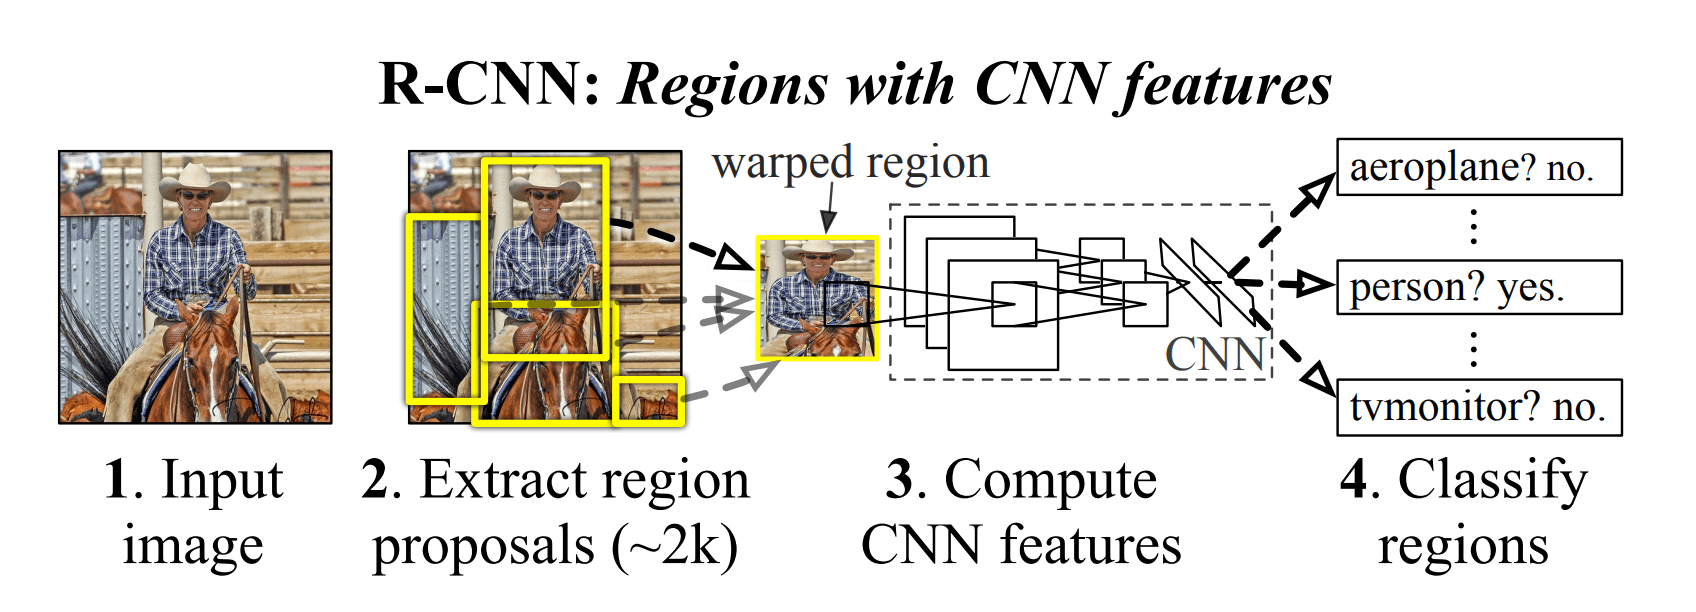
\includegraphics[width=.99\linewidth]{rcnn.png}
    \caption[Schéma fungování detektoru R-CNN]{Schéma fungování detektoru R-CNN. Ze vstupního obrazu~(1) jsou vyříznuty oblasti s~potenciálním výskytem objektů~(2). Z~těchto výsečí jsou pomocí konvoluční sítě~(3) získány příznaky, které jsou předány SVM klasifikátoru~(4). Obrázek je převzatý~\cite{paperRcnn}.}
    \label{fig_rcnn}
\end{figure}

Detektor \textbf{Fast R-CNN} tyto problémy řeší sdílením výpočtů konvolucí mezi jednotlivými okny s~objekty. Zároveň nahrazuje klasifikátor SVM vrstvou konvoluční sítě s~přechodovou funkcí softmax. Ke zlepšení výkonu také pomohlo použití sítě VGG16 oproti AlexNet~\cite{paperFastRcnn}.

Další iterace detektoru \textbf{Faster R-CNN} pak přinesla zdokonalení hledání podezřelých oblastí. Je jich nutné prohledat méně (asi~300 oproti~2000) a navíc je celý proces zrychlen. Autoři uvádějí zpracování až~5~snímků za sekundu na GPU~\cite{paperFasterRcnn}.

\textbf{Mask R-CNN} je detektor vyvinutý výzkumným týmem Facebooku a příchází s~něčím úplně novým. Oproti předchozím detektorům nepodává jako výstup souřadnice ohraničující objekt, ale provádí řazení do jednotlivých kategorií pro každý pixel obrazu~\cite{paperMaskRcnn}.

%-------------------------------------------------------------------------------

\subsection*{RetinaNet}

Model RetinaNet je na rozdíl od detektorů rodiny R-CNN jednostupňový. Avšak díky nové chybové funkci dosahuje přesnosti vyšší než jiné jednostupňové detektory (Single Shot Multibox Detector, Deformable Parts Model, You Only Look Once, ...). Je dokonce srovnatelný s~detektory dvoustupňovými~\cite{paperFocalLoss}.

Jeden z~problémů dosavadních jednostupňových detektorů je nevyrovnanost tříd (\textit{class imbalance}). Tyto detektory vyhodnocují mezi 10\,000\,--\,100\,000 možných výsečí pro každý vstupní obraz. Avšak jen velmi málo z~těchto výsečí skutečně obsahuje objekt. Poměr výřezů objektů vůči pozadí je až~1\,:\,1000~\cite{paperFocalLoss}. To má za následek, že většina výsečí je klasifikátorem snadno rozpoznána jako pozadí, respektive nerozpoznána jako žádný objekt. Trénování detektoru je při vysoké nevyrovnanosti tříd neefektivní. Většina výsečí jsou snadno rozpoznatelné negativní detekce, jelikož se jedná o~pozadí. Tento vysoký počet lehkých detekcí má za následek pomalé trénování případně dokonce degeneraci modelu. Detektor se totiž nejvíce učí z~těžkých dat, těch je ale malé množství v~porovnání se snadno identifikovatelným pozadí.

Autoři detektoru RetinaNet tento problém řeší novou chybovou funkcí \textbf{Focal loss}~\cite{paperFocalLoss}. Ta vychází z~chybové funkce Cross entropy (sekce~\ref{sec_training_neural_network}), která je široce využívaná jak u~jednostupňových tak dvoustupňových detektorů. Obohacuje ji o~parametr $\gamma$, pomocí kterého je možné korigovat váhu učení. Tvar chybové funkce v~závislosti na parametru $\gamma$ je zachycen na obrázku~\ref{fig_focal_loss}. Čím vyšší má hodnotu, tím více funkce zvýhodňuje učení z~obtížnějších, ale méně často se vyskytujících, dat.

\begin{figure}[H]
    \centering
    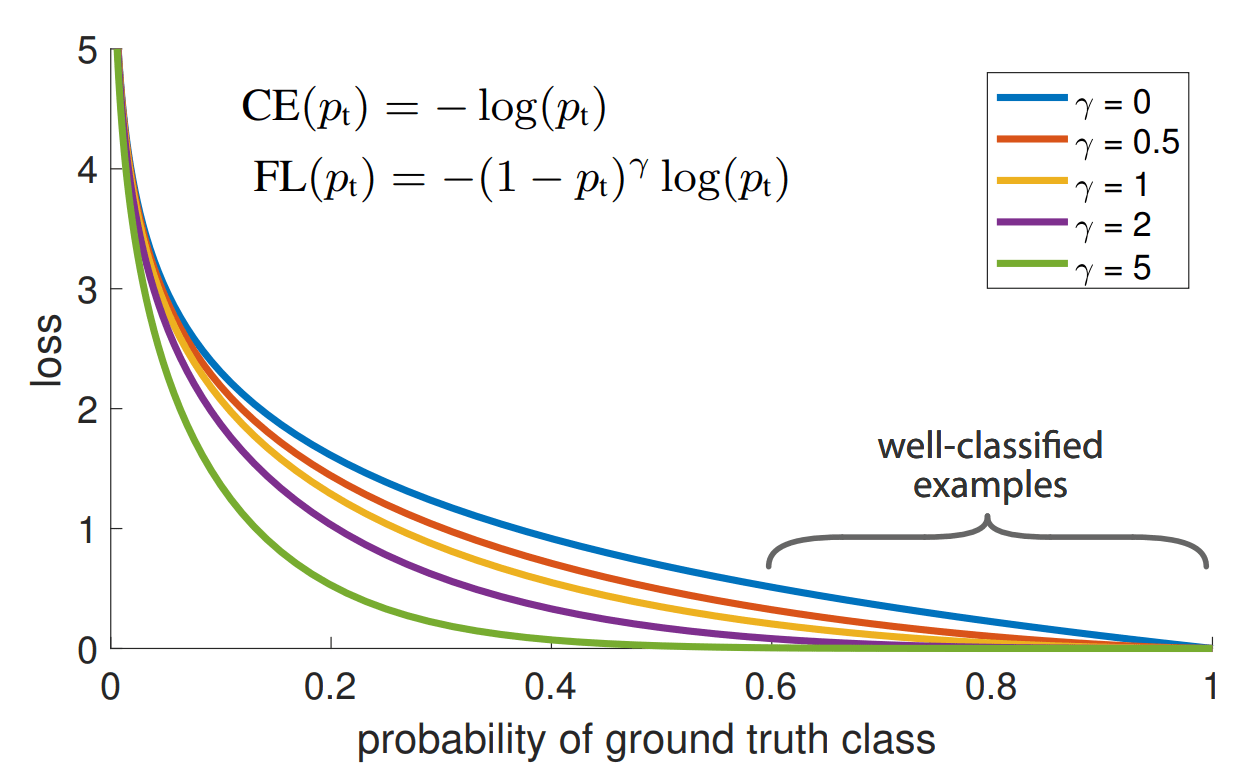
\includegraphics[width=.65\linewidth]{focal_loss.png}
    \caption[Chybová funkce Focal loss]{Funkce zachycuje hodnotu chybové funkce v~závislosti na pravděpodobnosti správně klasifikovaného objektu. Je-li parametr $\gamma$ roven~$0$, funkce je ekvivaletní s~Cross entropy. Obrázek je převzatý~\cite{paperFocalLoss}.}
    \label{fig_focal_loss}
\end{figure}

Detektor RetinaNet dále využívá strukturu \textbf{FPN} (Feature Pyramid Network)~\cite{paperFpn}. Ta pracuje se vstupním snímkem v~různých rozlišení a tím se snaží příznaky objektů zobecnit. Dokáže tak extrahovat slabé příznaky objektů zachycené v~nízkém rozlišení i silné příznaky objektů v~rozlišením vyšším (pyramida příznaků). Výsledkem je, že síť dokáže produkovat mapy příznaků v~různých škálách obrazu, což přispívá jak ke klasifikaci, tak k~regresi ohraničení.

\begin{figure}[H]
    \centering
    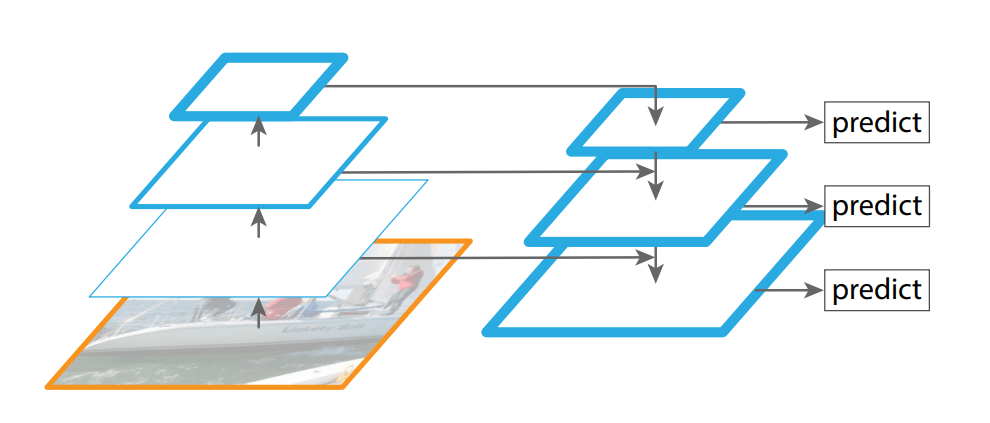
\includegraphics[width=.7\linewidth]{feature_pyramid_network.png}
    \caption[Schéma Feature Pyramid Network]{Příznaky jsou ze vstupního snímku extrahovány v~různém rozlišení a poté porovnávány s~příznaky pořízenými také v~různém rozlišení. Obrázek je převzatý~\cite{paperFpn}.}
    \label{fig_feature_pyramid_network}
\end{figure}

Je možné zvolit různé architektury konvolučních neuronových sítí pro klasifikaci (páteřní sít~--~\textit{backbone}). Často je využívána síť \textbf{ResNet} (Residual Network) od výzkumného týmu Microsoftu~\cite{paperResnet}. Jedná se o~jednu z~nejkomplexnějších architektur, která má ve svých variacích~50, 101~nebo až~152 vrstev. S~roustoucí hloubkou sítě by se přesnost teoreticky měla zvyšovat. Avšak s~roustoucí hloubkou je zpětně propagovaný signál od konce sítě k~jejímu počátku stále slabší. To ve výsledku znamená, že nižší vrstvy jsou učeny velmi málo či téměř zanedbatelně. ResNet tento problém řeší prostřednictvím tzv. zbytkových modelů (\textit{residual model}).

\begin{figure}[H]
    \centering
    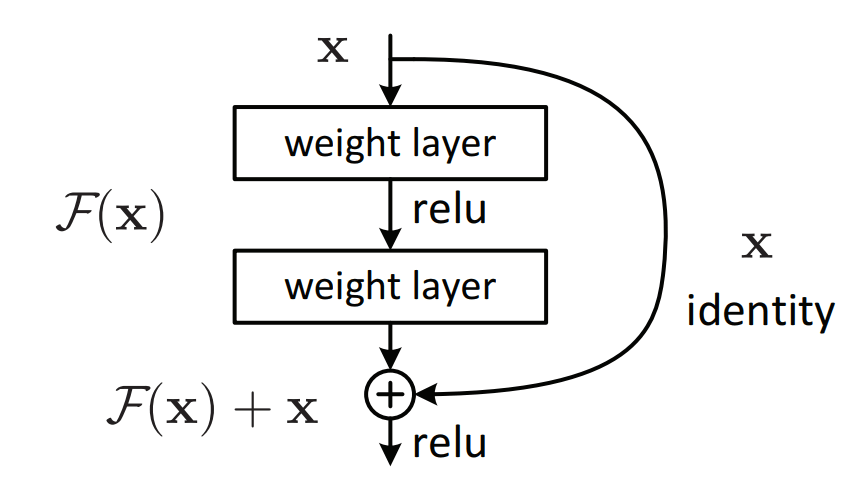
\includegraphics[width=.4\linewidth]{resnet-block.png}
    \caption[Zbytkový ResNet model]{Stavební blok zbytkového modelu. Obrázek je převzatý~\cite{paperResnet}.}
    \label{fig_resnet_block}
\end{figure}

Na soutěžním datasetu ILSVRC v~roce~2015 dosáhla ResNet chybovosti pouhých~3,57\,\%. Vzhledem k~faktu, že lidé dosahují chybovosti 5\,--\,10\,\% (v~závislosti na zkušenostech řešitele), se jedná o~výsledek, který se blíží maximální teoreticky možné úspěšnosti~\cite{paperResnet}.

\begin{figure}[H]
    \centering
    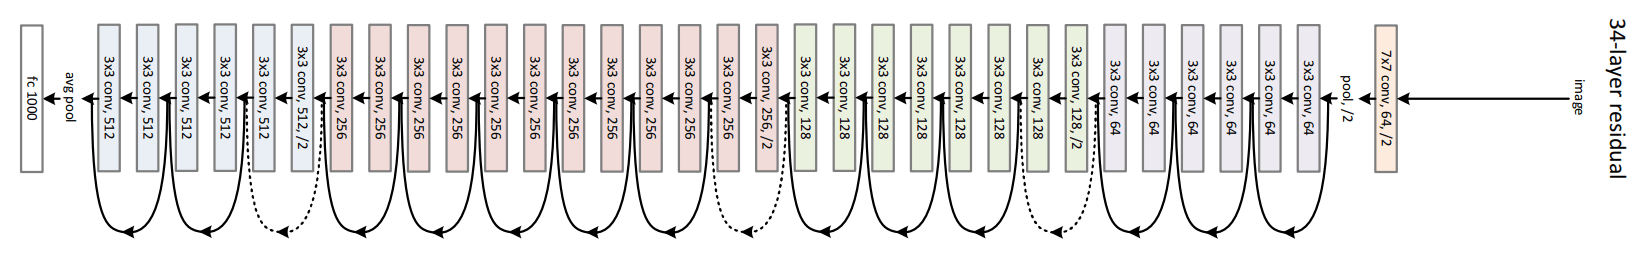
\includegraphics[width=.99\linewidth]{resnet-architecture.png}
    \caption[Architektura sítě ResNet]{Architektura ResNet se znázorněním konceptu zbytkových modelů. Obrázek je převzatý~\cite{paperResnet}.}
    \label{fig_resnet_architecture}
\end{figure}

%-------------------------------------------------------------------------------

\subsection*{Výběr detekční sítě}

Dvě hlavní kritéria ovlivňující výběr detekční sítě jsou přesnost a rychlost detekce. V~oblasti rychlosti si práce neklade velké cíle, není účelem dosáhnout detekce v~reálném čase (\textit{real-time}). Detektor bude detekovat osoby z~výšky z~pohledu ze shora. To může být poměrně náročný úkol. Jak je představeno v~sekci~\ref{sec_dataset}, člověk z~výšky je snadno zaměnitelný objekt. Vzhledem k~typu objektů, které detektor bude detekovat, je přesnost daleko významnější kritérium.

Na obrázku~\ref{fig_detectors_comparision} je vidět, že detektor RetinaNet překonává v~přesnosti ostatní algoritmy~\cite{articleDetectorsComparision}. Alespoň v~měřeních na složitých datech z~datasetu COCO. Navíc zachovává rozumnou rychlost detekce. Proto je vhodným detektorem pro účely této práce.

\begin{figure}[H]
    \centering
    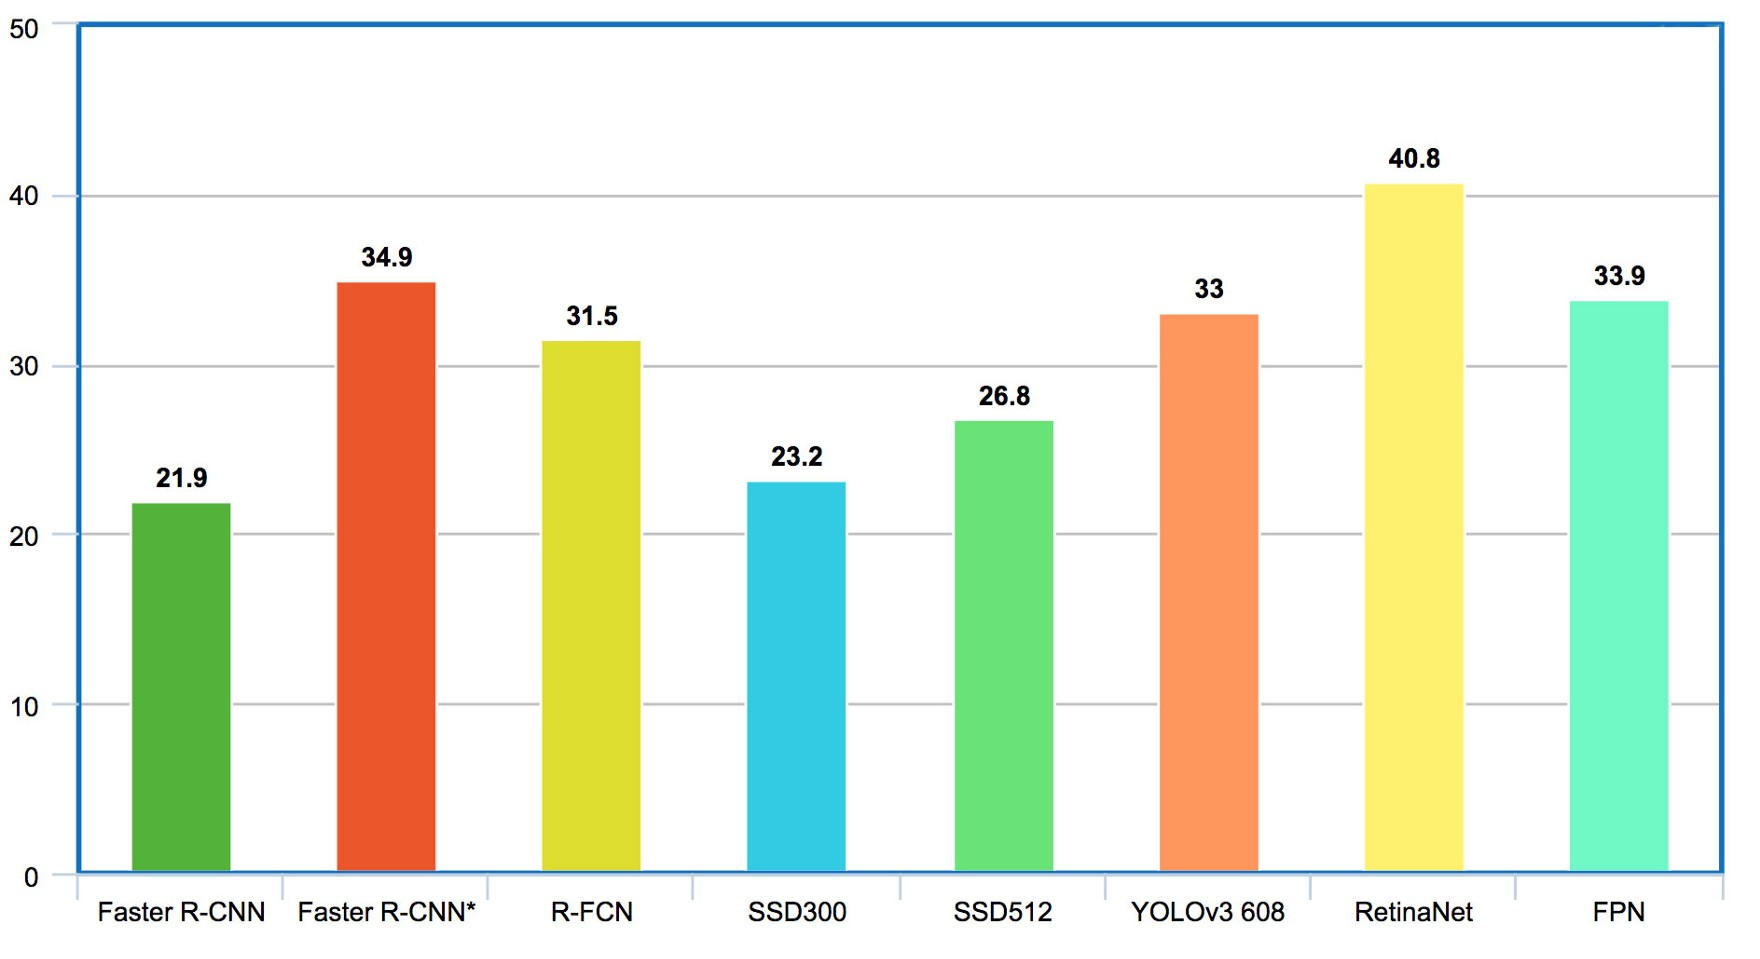
\includegraphics[width=.99\linewidth]{detectors_comparision.jpg}
    \caption[Porovnání přesnosti několika různých detektorů]{Porovnání přesnosti několika různých detektorů na datasetu COCO. Pro oblast detekce objektů se jedná o~složitější dataset, proto detektory dosahují relativně nízké přesnosti. Obrázek je převzatý~\cite{articleDetectorsComparision}.}
    \label{fig_detectors_comparision}
\end{figure}

%===============================================================================
